
\graphicspath{{ChapterTexture/images/}}
%% Chapitre I %%
\chapter{Texture synthesis for 3D object representation}
\label{chapter:textureSynthesis}

\section{Introduction}

A texture synthesis approach will be used to enhance the properties of objects. 
The objective in this dissertation is to produce solid blocs of physical parameters. 
These solids will be used with s-reps to produce simulated images.
To understand this approach, it is necessary to 
understand the properties of texture.

Objects in the real world have a large number of visual properties.
Among those properties are luminance, color, relative motion, stereo disparity
and surface characteristics including reflectance and roughness.
When all of them are combined, the result is a textured image. 

Human perception has the capability to separate textured regions.
This phenomenon is known as texture segregation;
it allows us to distinguish a wide variety of objects and materials with little effort.

Figure \ref{fig:textureSegregation} shows an image composed by 
three types of letters $Xs$, $Ts$ and $Ls$. We are able to easily detect
the left region ($Xs$) but some effort is required to differentiate
the right region ($Ts$) from the background ($Ls$). 
Even though there are no clear edges in the image, our visual 
system is capable of detecting all of the regions.
\begin{figure}
  \centering
  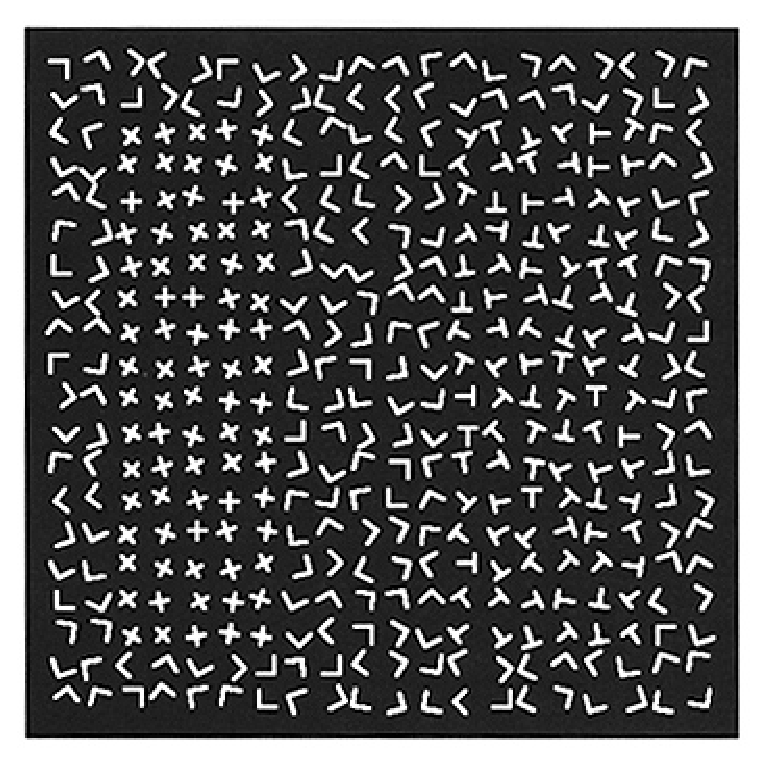
\epsfig{file = textureSegregation.eps, width = 8cm}  
  \caption[Texture segregation.]{Image taken from \cite{bergen1991computational}. 
	   The image has three regions that can be distinguished: 
	   One composed by $Xs$ a second one with $Ts$ and the background with $Ls$.}
 \label{fig:textureSegregation}  
\end{figure}

This type of observation led to the \textit{Julesz conjecture}, a hypothesis 
as to whether human texture perception was sensitive only to differences 
in the first %order statistics (mean, variance, skewness, kurtosis) 
and second order statistics. % (angular second moment, contrast, correlation, homogeneity, entropy).
It was later concluded by Julesz himself that images with identical third order statistics 
could also be easily discriminated by our visual system \cite{julesz1978visual}. 

The counterexamples gave the idea that it was possible to model texture with low-order statistics
and led to feature-based theoretical approaches.

\begin{definition}
 Textons are fundamental micro-structures in generic natural images and the basic elements in early (pre-attentive) visual perception.   
\end{definition}

Texture analysis by its features or textons
enabled the reduction of redundant information and produced compact 
representations of texture easier to manipulate.
This characterization found application in a wide variety of fields that include
image segmentation and object recognition \cite{leung2001representing},
and image/video editing, merging, and completion \cite{wexler2004space}.
It provided cues to understand the function of neurons in biologic vision systems
which led to advances in neurophysiological 
texture perception \cite{olshausen1997sparse}, \cite{landy2004visual}.

In computer graphics, applying textures to geometric models
is key to enhance 3D object representation. 
As texturing and rendering methods improve, 
3D virtual objects become more realistic 
and appealing to our visual system. 

The first step to apply texture in a 3D object is to acquire 
samples large enough to cover their whole surface.
To do this, we need methods capable of synthesizing texture. 

Textures can be categorized in a structural vs. stochastic tradeoff. 
Natural textures are found 
somewhere in between containing stochastic and regular aspects. 
Structural textures have regular patterns such as a tiled floor.
Stochastic textures don't have a specific structure or organization; they look 
like colored dots randomly distributed in the image. 
In general, there are two approaches to synthesize texture. Procedural 
and exemplar-based.

Procedural approaches seek to model texture using noise functions.
These methods exploit the stochastic features of textures and 
a wide variety of results can be achieved by ``structuring'' the noise.

On the other hand, exemplar-based approaches rely on the MRF (Markov Random Field)
assumption, \emph{i.e.}, texture locality and texture stationarity. 
Assume that we are able to analyze a textured image using small windows of fixed size. 
Texture locality means that new pixels could be predicted from 
the information on a single spatial window
and texture stationarity means that texture spatial statistics are invariant 
in multiple windows. 
This line of thought has many desirable properties. 
It suggest that a small textured sample can be used to 
replicate the stochastic and structural features on larger images. 
The major drawback would be the time to synthesize a result.

The first challenge of MRF approaches is to
keep the initial look of the exemplar.
This can be done by replicating the texture features at random places in 
the new image while avoiding unnatural seams and repetitions.
A second challenge is to synthesize texture on a surface using properties 
such as orientation or scale.

In this dissertation,
a MRF approach for solid texture synthesis is used.
Solid textures provide volumetric information 
and model internal properties.
They can be used to perform scattering simulations,   
enhance volume rendering of an object or reveal
internal features.
In the same manner, the synthesis method uses 2D textured images
and produces a solid with similar characteristics to the exemplar.

Solid textures will be used on organ models
to generate solids representing
the parameters for MRI image simulation. 
These parameters are obtained using relaxometry. A technique that measures 
specific physical and chemical properties of materials in MRI.
Besides generating distributions of physical parameters,  
the synthesis method can be used 
to improve the visual properties of objects. 

%After a RF (radio frequency) pulse is applied to a system it puts the nuclei in a high energy state. 
%Relaxometry measures the time in which the system relaxes or returns to equilibrium. 
%The acquired values are $T1$, $T2$, $T2^*$ and $\rho$ (proton density).
%$T1$ and $T2$ are relaxation constants measuring the spin lattice and spin spin relaxation time,
%$T2*$ measures the local field inhomogeneity and $\rho$ is the proton density or 
%concentration of mobile hydrogen atoms within the tissue. 

Exemplar textures are generated for some brain structures 
containing the corresponding physical parameters
acquired in the relaxometry images. 
The textures have four channels: $T_1$, $T_2$, $T_2^*$ and $M0$, 
\textit{i.e}, two relaxation constants, the local field inhomogeneity and proton density. 
The generated textures applied on the geometric models 
will be used to simulate an image of some brain structures,
the simulation is explained in Chapter \ref{chapter:MRISimulation}.
%The solid textures can be applied to geometric models, 
%enhancing their internal properties. 

The following section reviews the most important authors for 
procedural and exemplar-based texture synthesis.

\section{Texture synthesis methods and applications}

\subsection{Procedural texture synthesis}

Procedural texture synthesis methods are useful to simulate elements from nature 
like clouds or water waves. 
They are memory-efficient and guarantee continuity and consistency of the texture.
In theory, procedural approaches 
can generate any pattern but the calibration of the method can be a very difficult task. 
The procedure is not intuitive since the user must elaborate an analytic description of the texture.

Solid textures can be synthesized by procedural methods
\cite{perlin1985image} and \cite{peachey1985solid}.
In fact, the functions return
a color value at any given point in 3-space.

Different texture patterns have been studied.
\cite{witkin1991reaction} used a reaction-diffusion equation to generate 
stripe patterns.
\cite{walter2001integrating} used a biological model
to reproduce the texture of animal skin.

A recent approach by \cite{lagae2009procedural}
is able to generate several
natural textures like marble, wood and
different animal skin patterns. It provides 
a user-friendly interface to set up the required parameters 
to control how the texture is generated. 
Controlling the noise patterns allows texture generation according 
to surface orientation; in other words, a fiber-like texture
can be oriented on the object's surface and no object-coordinates are needed.

The advantages of procedural texture synthesis are that
it does not require much memory to synthesize the texture; 
that the resolution is not fixed and detail can be added depending on the scale;
that it can cover large areas without seams or texture repetitions;
and that it can be parameterized to generate a transition to a different texture during the procedure.

\subsection{Exemplar based texture synthesis}

In this dissertation, an exemplar-based method is used to generate solid textures. 
The reasons are that procedural textures
are difficult to build and it is hard to control how the patterns are generated.
Exemplar-based approaches provide more flexibility to be used with 
different textures in the stochastic - structured range. 

For the rest of the chapter the following definition of texture synthesis is used:

\begin{definition}
 Texture synthesis is the process of generating a larger textured image from a small exemplar.
\end{definition}

Exemplar-based synthesis usually has two stages: 
a search in the texture sample space and a merge phase to produce the 
synthesized output. Most of the methods have also been extended to
synthesize solids.

\subsubsection{Pixel-based synthesis}

The texture synthesis approach proposed by \cite{efros1999texture}, 
starts with a seed pixel and 
grows outwards. 
It performs a closest neighborhood 
search in the sample image
and then it grows by adding new pixels accordingly. 
To achieve good results with textures such as a brick wall,
it is necessary to employ large neighborhoods in order to capture 
the structure of the texture. 
Moreover, the search step does not enforce using
all of the texture information in the image and causes 
repetition of the same neighborhoods very often.

\cite{wei2000fast} proposed some improvements that modified
the search step using a fixed size neighborhood and a random initialization of the output texture. 
The fixed neighborhood allowed data structures such as kd-trees to accelerate the search phase and
allowed the random initialization enforced in the synthesis to use 
more information from the exemplar. 
Unfortunately, the method is highly dependent on 
the initialization stage and in some cases is not able to 
include all the information from the exemplar. 

\cite{ashikhmin2001synthesizing} proposed 
a speedup based on coherence. The idea is to keep
the positions on the exemplar of the synthesized pixels.
It is unlikely that pixel chosen during the synthesis 
will change to a different one.
Therefore, keeping the index position reduces the overall search time to produce an output. 
\cite{tong2002synthesis} further improved coherence by 
keeping $k$ candidate pixels. The $k$-coherence approach produces the best results among
the pixel based methods. 


\subsubsection{Patch-based synthesis}

Patch-based synthesis is similar to pixel-based approaches. 
The difference is that instead of writing a single pixel, a whole patch is written to the result. 
Some techniques conceived to produce a good result when merging patches are
the following:
overwrite the overlapping patch \cite{praun2000lapped};
blend the overlapping regions \cite{liang2001real};
find an optimal cut to seam the patches \cite{kwatra2003graphcut};
and warp the patches to ensure continuity \cite{wu2004feature}.

There are some known issues about these techniques. 
Blending the patches might cause blurring ,
and when the smooth transition between regions is not found,
the output textures contain visible seams.

In general, pixel- and patch-based approaches 
are prone to accumulate small errors 
over the synthesis procedure and lead to 
inconsistencies in the synthesized texture.

\subsubsection{Optimization-based synthesis}

Texture synthesis by optimization was proposed by \cite{kwatra:2005:SIGGRAPH}.
The approach uses the best of both techniques previously discussed. 
It calculates the output value one pixel at time, but it
uses the information from all of the patches that contribute 
to a single pixel. 
The value is determined by optimizing a 
quadratic energy function, leading to better output quality.

The global optimization framework is designed from 
an MRF assumption. If locality and stationarity are 
satisfied, a global measure of energy can 
be designed by comparing the neighborhoods 
of the input and output textures. 
The energy is defined as the distance to the
closest neighborhood in the exemplar.
The sum over all neighborhoods defines the total energy of the output texture,
and the solution of the synthesis procedure is found when 
the energy is minimized. 

Texture synthesis by optimization is very flexible. 
It has the advantage of creating models using one or multiple samples 
in order to constrain the view perpendicular to each axis direction.
It can use multi-channel textures like RGB and distance maps \cite{Lefebvre:2006:ATS:1141911.1141921}. 
%to code large unstructured areas \cite{Lefebvre:2006:ATS:1141911.1141921}.
\cite{KFCODLW07} improved the optimization procedure by adding 
histogram matching and enforcing the exemplar statistics on the volume.
\cite{chen2010high} uses index and position histograms to 
enforce the synthesis procedure to use all neighborhoods from the exemplar. 

\subsection{Enhancing medical applications using textures}

Texturing anatomical structures of the body has been used to 
understand complex medical images and distinguish 
organ details such as orientation, scale and materials \cite{netter2010atlas}.

This type of illustration is used to facilitate the communication process 
among doctors, students and patients. 
Medical students use these illustrations to facilitate the learning and training process.
Doctors and surgeons use them to explain a certain treatment to a patient.
However, it is desirable to have this information using patient-specific
data since the shape of an organ may vary depending 
on the phenotype or pathology from one patient to another. 
Moreover, patient-specific illustrations can be used to guide subsequent 
treatment and planning to an optimal direction; notably dose radiation 
for cancer treatment needs high quality patient-specific models.

\cite{merck2009model} proposed MGR (model guided rendering). It seeks 
to enhance patient-specific anatomical models
using textures and provides the mechanism 
to improve radiotherapy planning. 
\cite{kabul2011optimal} improved the mechanisms to apply texture 
to organ models by controlling the synthesis procedure using vector 
fields and texture metamorphosis.
Texture metamorphosis refers to the process of smoothly interpolating between two
textures. 

MGR uses the coordinate system provided by m-reps (see Section \ref{sec:medialRepresentations}) 
and applies solid textures to the models according to their geometric 
properties.
The following section explains the technique to synthesize solid textures.

\section{Solid texture synthesis}
\label{sec:solidTextureImplementation}
\begin{figure*}
 \centering 
 %\subfigure[]{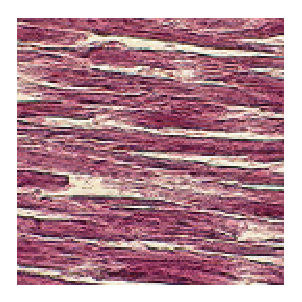
\epsfig{file = skeletal_muscle.eps, width = 1.6cm}}
 \subfigure[]{
\epsfig{file = striescardiaques.eps, width = 2cm}}
 \subfigure[]{
\epsfig{file = myocyte.eps, width = 2cm}}
 %\subfigure[]{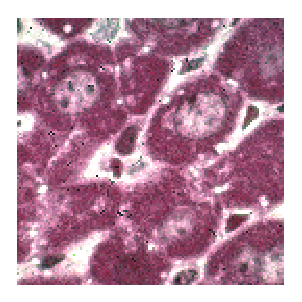
\epsfig{file = hepatocyte.eps, width = 1.6cm}}
 \subfigure[]{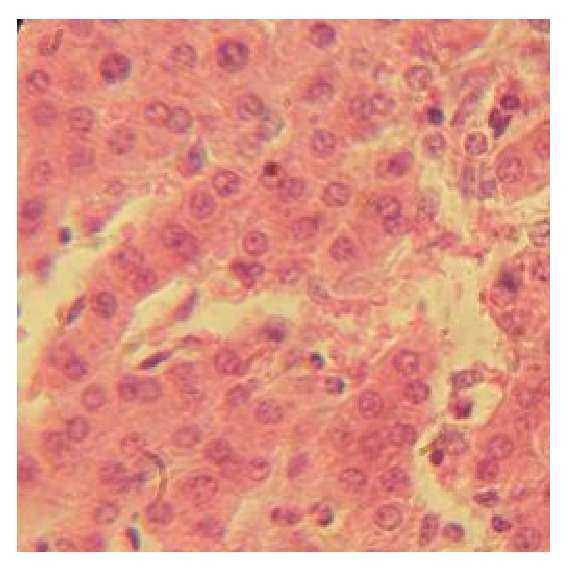
\epsfig{file = hepatique.eps, width = 2cm}}
 \subfigure[]{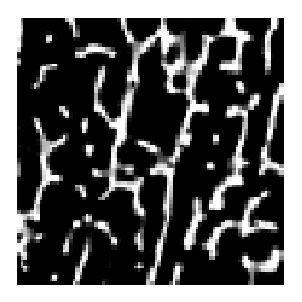
\epsfig{file = esrf.eps, width = 2cm}}
 \subfigure[]{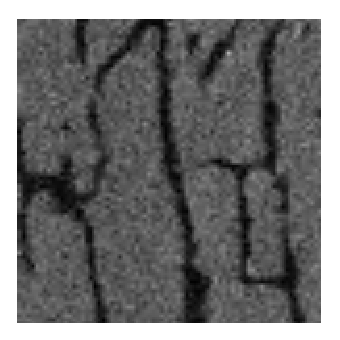
\epsfig{file = vol.73-93-94-sliceX.eps, width = 2cm}} 
 \subfigure[]{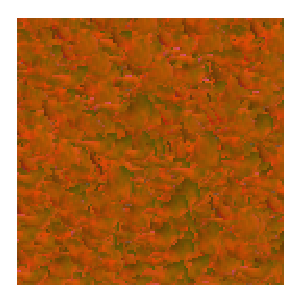
\epsfig{file = Left_HippocampusPhysicalParams.eps, width = 2cm}}
 \caption[Exemplar textures.]{$128^2$ textured samples available to create volumetric data: 
          histology images of (a) striated cardiac muscle, (b) myocytes, 
	  (c) hepatocytes; (d - e) a slice from a SR$\mu$CT and $\mu{MR}$ image of a trabecular bone sample; (f) physical parameters image of the hippocampus 
	  ($T_1$-red, $T_2$-green, $T_2^*$-blue, $M0$-alpha. All channels rescaled between [0-255] for illustration purposes).
          }
 \label{fig:sampleimages}
\end{figure*}


The interior of organs must be textured to make them 
appear as if they were the physical parameters required for MRI simulation.
The solid texture synthesis method derives from \cite{KFCODLW07}. Similarly, the method uses exemplars and 
by means of an energy optimization process, the 3D texture looks like the 2D image in every slice.
This implementation has been reviewed in \cite{PRIE-12a}, \cite{PRIET-12b}, \cite{PRIE-11}.
The reference image can be textured elements from different sources such as: 
\begin{enumerate}
 \item Artificial images artistically created for computer graphic design or medical atlases.
 \item Real images from digital microscopy of biomedical histological slices.
 \item 2D reference textures provided by slices extracted from a $\mu{MR}$ and $SR \mu{CT}$.
 \item Textured images of physical parameters required to perform MRI simulation (the image is rescaled for visualization purposes). 
\end{enumerate}
Figure \ref{fig:sampleimages} shows some examples of texture. 

Section \ref{sec:TextureSynthesisResults} presents the generated solids with the exemplar images shown in Figure \ref{fig:sampleimages}. 

Modeling different types of organs and tissues at the cellular level represents an interest for histology, 
\emph{i.e.}, the study of tissues. Histology plays an important role in the comprehension of 
morphological relationships between the organs and tissues. It considers the structural organization 
or precise hierarchy of the organs with the smallest details. 
When a geometric model is enhanced with these type of textures, 
it will acquire structural information at different scales.

The approach is based on the optimization framework proposed by \cite{kwatra:2005:SIGGRAPH} 
defined by the following equation:

\begin{equation}
 E(o, \{e\} ) = \sum_{t} \sum_{i \in \{x, y, z\}} \sum_{u \in N_i(t)} w_{t, i} ( o_{t, i, u} - e_{t, i, u} )^2
 \label{equ:imagenergy} 
\end{equation}
\begin{equation}
 w_{t,i} = || o_{t, i} - e_{t, i} ||^{-1.2}
 \label{equ:neighweight}
\end{equation}

Equation \ref{equ:imagenergy} calculates the distance between the $x$, $y$ and $z$ neighborhoods 
of a texel $t$ in the object $o$ to the collection of 2D neighborhoods of the exemplar texture $e$. 
Equation \ref{equ:neighweight} shows how to calculate the weight given to each neighborhood.
The coefficient $-1.2$ is used to perform a robust optimization \cite{kwatra:2005:SIGGRAPH}.
When this function is minimized using IRLS (iterative re-weighted least squares), 
the result is an increase of similarity between the sample and the synthetic object.

The procedure begins at a coarse resolution assigning random values from the sample to the synthetic object. 
It alternates between a search phase, where the closest neighborhoods are found,
and an optimization phase, where the weighted average of every texel is calculated. 
When the optimization converges, it changes to a finer resolution level using linear interpolation.

The following section gives details about the implementation.
Section \ref{sec:TextureSynthesisResults} shows the volumes and Section \ref{sec:EvaluationTexture}
evaluates the quality of the synthesized texture. 

The accuracy of the synthetic images is assessed and discussed by comparing statistical and morphological parameters computed from the virtual and the real images.

\subsection{Search phase}
\label{sec:SearchPhase}

\begin{figure}[!h]  
  \centering
  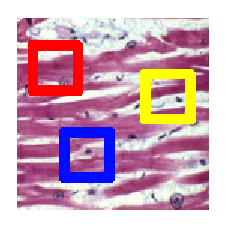
\epsfig{file = search_sample.eps, width = 3cm}
  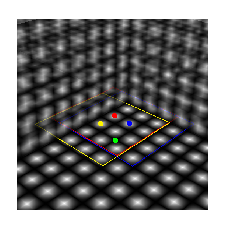
\epsfig{file = search_phase.eps, width = 6cm}
  \caption[Texture synthesis neighborhoods.]{9x9 red, blue and yellow neighborhoods for a slice in the volume, the center is represented by the colored dot.
           The green voxel is affected by multiple neighborhoods.}
  \label{fig:search_phase}  
 \end{figure}

The sample image is divided into $9 \times 9$ neighborhoods that overlap each other. 
These neighborhoods are vectorized, \emph{i.e.},
every texel from the neighborhood is stacked into a single vector. 
For RGB texels we have $9 \times 9 \times 3 = 243$ values in a single vector. 

Once the vectors from the sample are constructed, PCA (see Appendix \ref{sec:apendixPCA})
reduces the dimensionality of each vector passing from $243$ to $18$ values approximately.
Reducing the vectors is a very convenient step, there are less values but we are still keeping $95\%$ of the relevant information.
The reduced vectors can be used to perform a standard closest neighborhood search in a high dimensional space. 
The ANN library\footnote{ANN: A library for approximate nearest neighbor searching; \url{http://www.cs.umd.edu/~mount/ANN/} Mount, D. M. and Arya, S. 2006}
is used for this purpose.

During the search phase, a weight for each neighborhood is calculated. 
The energy function is written as shown in Equation \ref{equ:imagenergy}.
The weight of each neighborhood is calculated as shown in Equation \ref{equ:neighweight}. 
$N_i(t)$ represents the neighborhoods for each dimension $x$, $y$, $z$ 
and $u$ is the texel in the neighborhood of $t$. 
This means that a texel in the object is affected by multiple texels from different neighborhoods in the exemplar texture. 
The search is performed for every two texels $g_x = \{(i, 2 \times j, 2 \times k), \forall i, j, k \}$ 
($g_x$ is the voxel in a slice perpendicular to $x$). 
This is done similarly for $y$ and $z$, as shown in Figure \ref{fig:search_phase}.

Once the search phase is done the optimization phase takes place and it consists in averaging 
all the values found for each texel of the volume. 

\subsection{Optimization phase}
\label{sec:OptimizationPhase}

The optimization phase consists in averaging the values that affect one texel in the object. 
If the search phase is performed for every two texels as in \ref{sec:SearchPhase}, 
the average will be for at most 75 texels (25 for each dimension).

\begin{equation}
 o_t = \frac{ \sum_{i \in \{x, y, z\}} \sum_{u \in N_i(t)} w_{u, i, t} \times e_{u, i, t} }{ \sum_{i \in \{x, y, z\}} \sum_{u \in N_i(t)} w_{u, i, t} }
 \label{equ:texelaverage}
\end{equation}

Equation \ref{equ:texelaverage} shows the value of a texel in the object. 
When the texels present a high variability, the resulting object might be
blurred. In order to avoid this issue, 
clustering is performed to only average those texels that correspond to the principal cluster.

After the optimization phase, histogram matching is done. 
This method preserves the global statistics of the exemplar in the synthetic object.
As explained in the following section.

\subsection{Histogram Matching}
\label{sec:histogramMatching}

This method maintains the global statistics of the sample by using a histogram matching approach \cite{ROLLAND2000}, \cite{Heeger:1995:PTA:218380.218446}.
To perform histogram matching, the $CDF$ (cumulative distribution function) of the histograms 
is calculated for both the exemplar and the object. 
Two $LUTs$ are constructed in order to perform faster calculations. 
The lookup table $LUT_o$ maps the RGB values of the object
to their corresponding value in the $CDF_o$. 
The lookup table $LUT_e$ maps the $CDF_e$
to the corresponding RGB values from the sample. 
The object is then modified by taking each of the texels $t$ and using $LUT_o(t)$ to find the $CDF_o(t)$.
Using $LUT_e(CDF_o(t))$ finds the corresponding RGB value from the sample. 
The value of the object is replaced by the corresponding value in the exemplar.

%\begin{figure}[!h]  
%  \centering
%   {\epsfig{file = histogramCDFLUT.eps, width = 5.5cm}}
%  \caption{CDF of the exemplar and the object with the corresponding $LUT$ functions.}
%  \label{fig:histogramMatch} 
%\end{figure}

The following section shows some results produced by the implementation of the 
texture synthesis algorithm. 

\section{Types of solid textures}
\label{sec:TextureSynthesisResults}

%The algorithm was implemented in C++ using ITK\footnote{\url{http://www.itk.org}} for image processing and 
%VTK\footnote{\url{http://www.vtk.org}} for visualization. 
%Using ITK allowed the image processing to be performed in parallel, thus gaining computational time.
%Synthetic 3D images of both $128^3$ pixels and $256^3$ pixels were generated using different type of textures, from histology images 
%acquired with a digital microscope.% and image samples from IRM image acquisitions. 

\subsection{Isotropic texture from a 2D exemplar texture}

\begin{figure}[h!]
 \centering
 \subfigure[Striated cardiac tissue.]{
            
\epsfig{file = striescardiaques.eps, width = 2cm} 
	    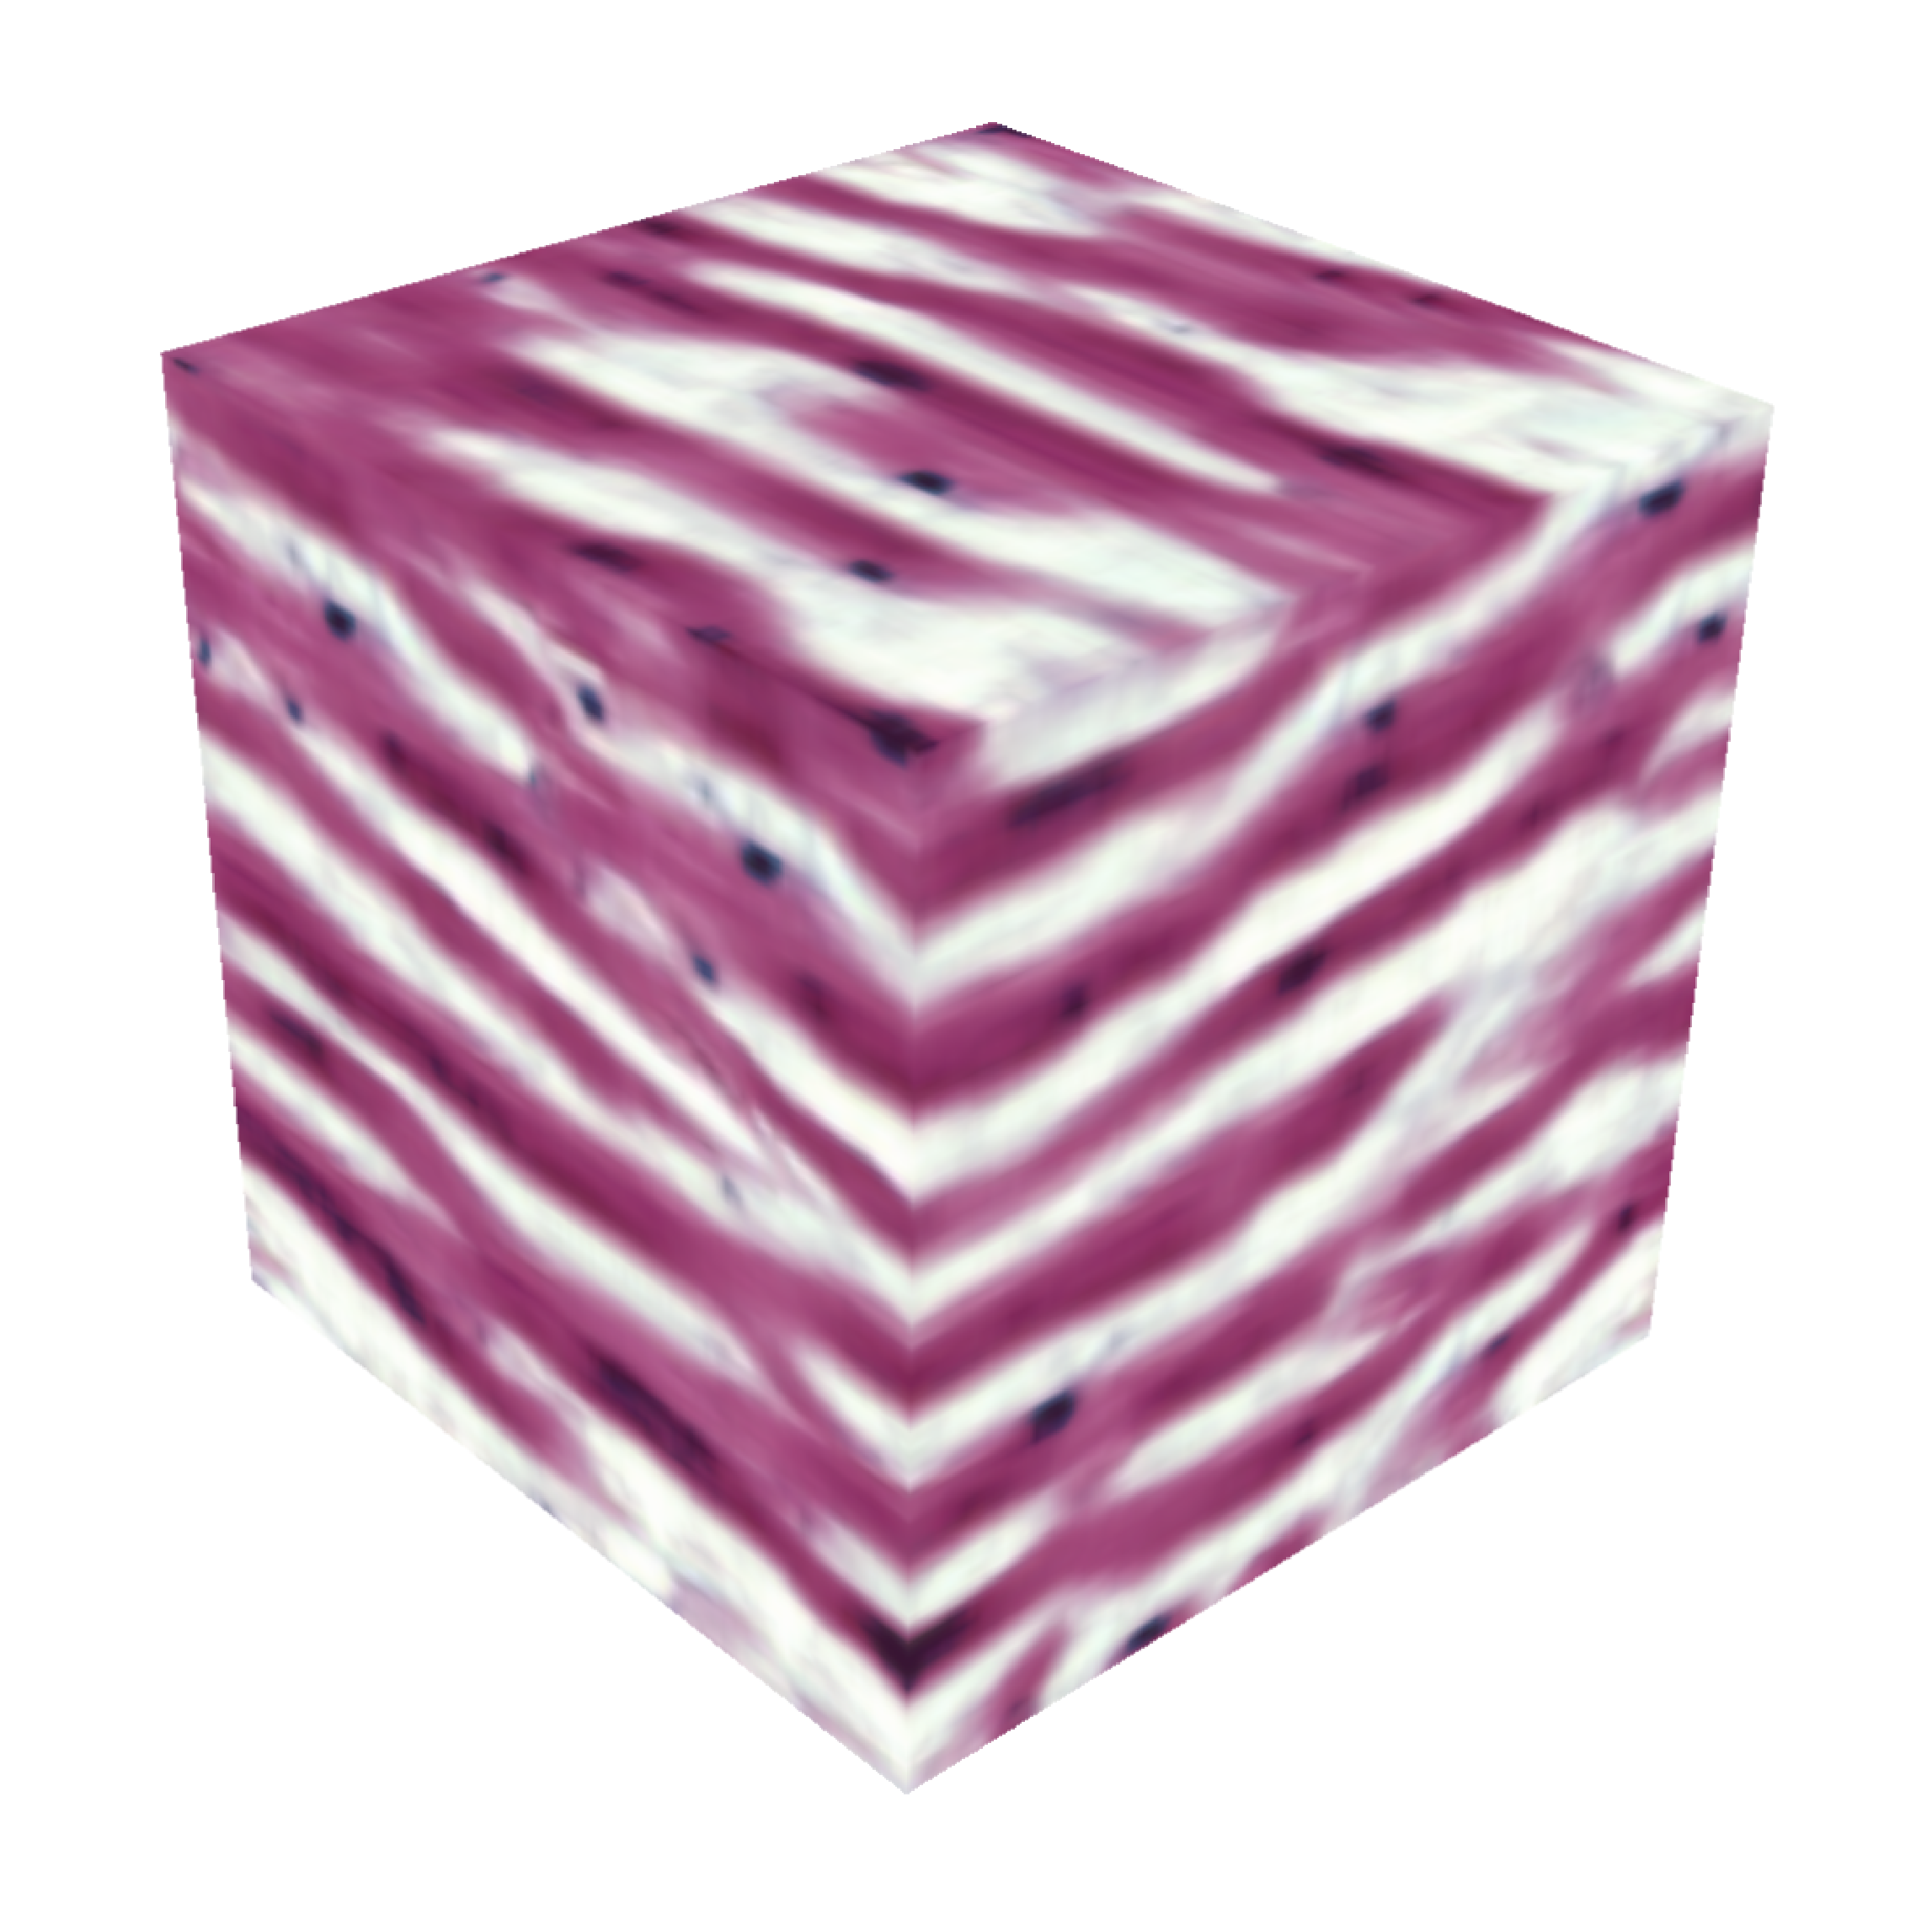
\epsfig{file = striescardiaquesVol.eps, width = 5cm}
	    }
 \subfigure[Liver cell tissue.]{
	    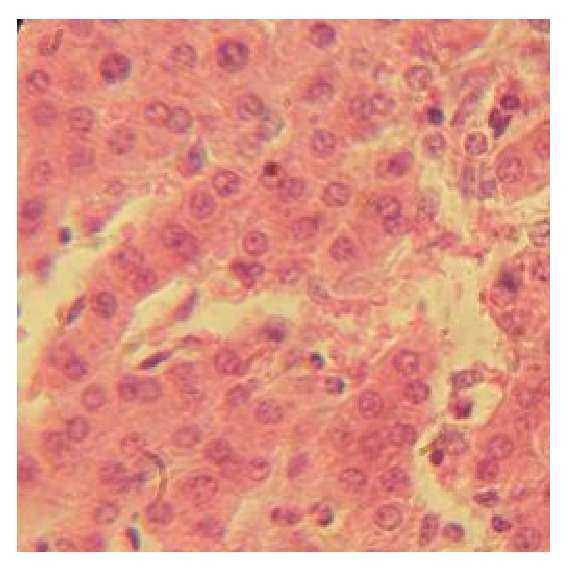
\epsfig{file = hepatique.eps, width = 2cm}
	    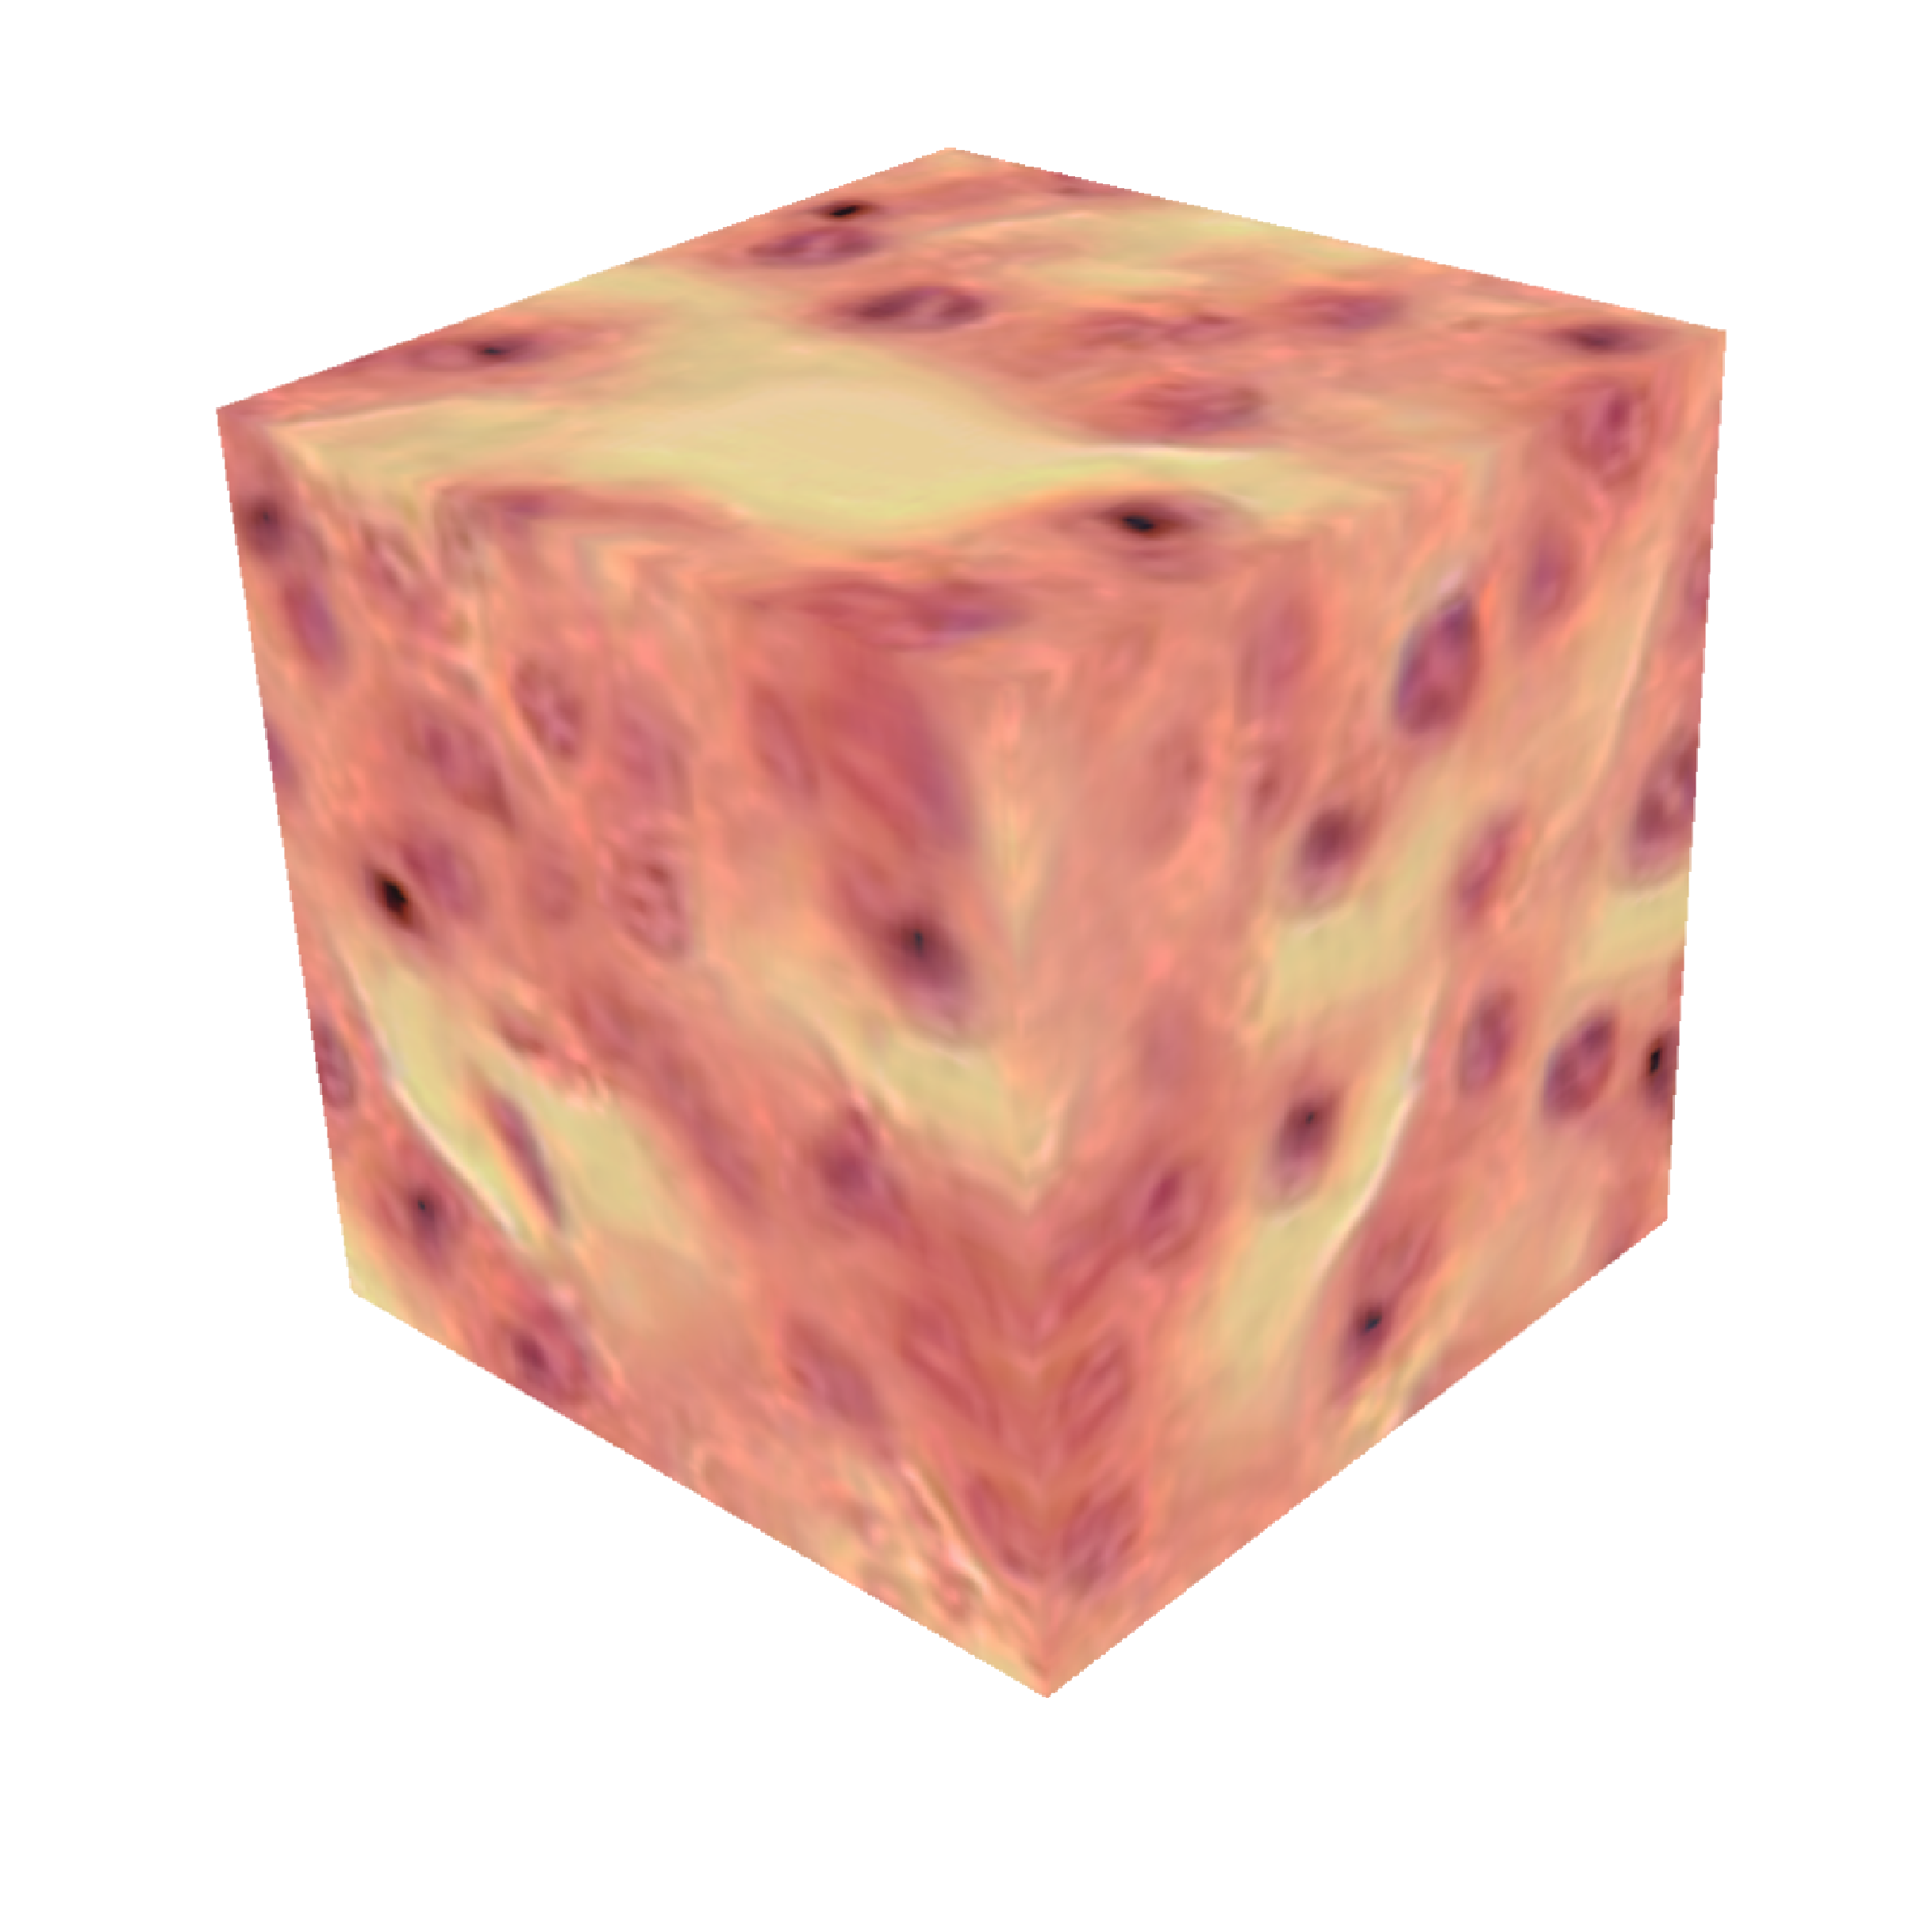
\epsfig{file = hepatiqueVol.eps, width = 5cm}
	    } 
 \caption[Isotropic texture synthesis.]{Results of isotropic synthesis. The striated cardiac muscle tissue (left)
          and liver cell tissue (right) were generated using a single reference texture 
          for the axial, longitudinal and transversal planes.
         }
 \label{fig:isotropicsynthesis} 
\end{figure}

Figure \ref{fig:isotropicsynthesis} shows some results when the same exemplar is used to constrain 
the axial, longitudinal and transversal planes.
The method produces a volume of striated 
cardiac muscle tissue and the liver cell tissue from histology.
Every longitudinal or transversal slice of the volume is similar to the reference texture without being, however, identical.

\begin{figure}[h!]
 \centering
 \subfigure[Hippocampus' physical parameters]{
            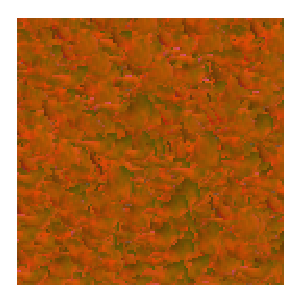
\epsfig{file = Left_HippocampusPhysicalParams.eps, width = 2cm} 
	    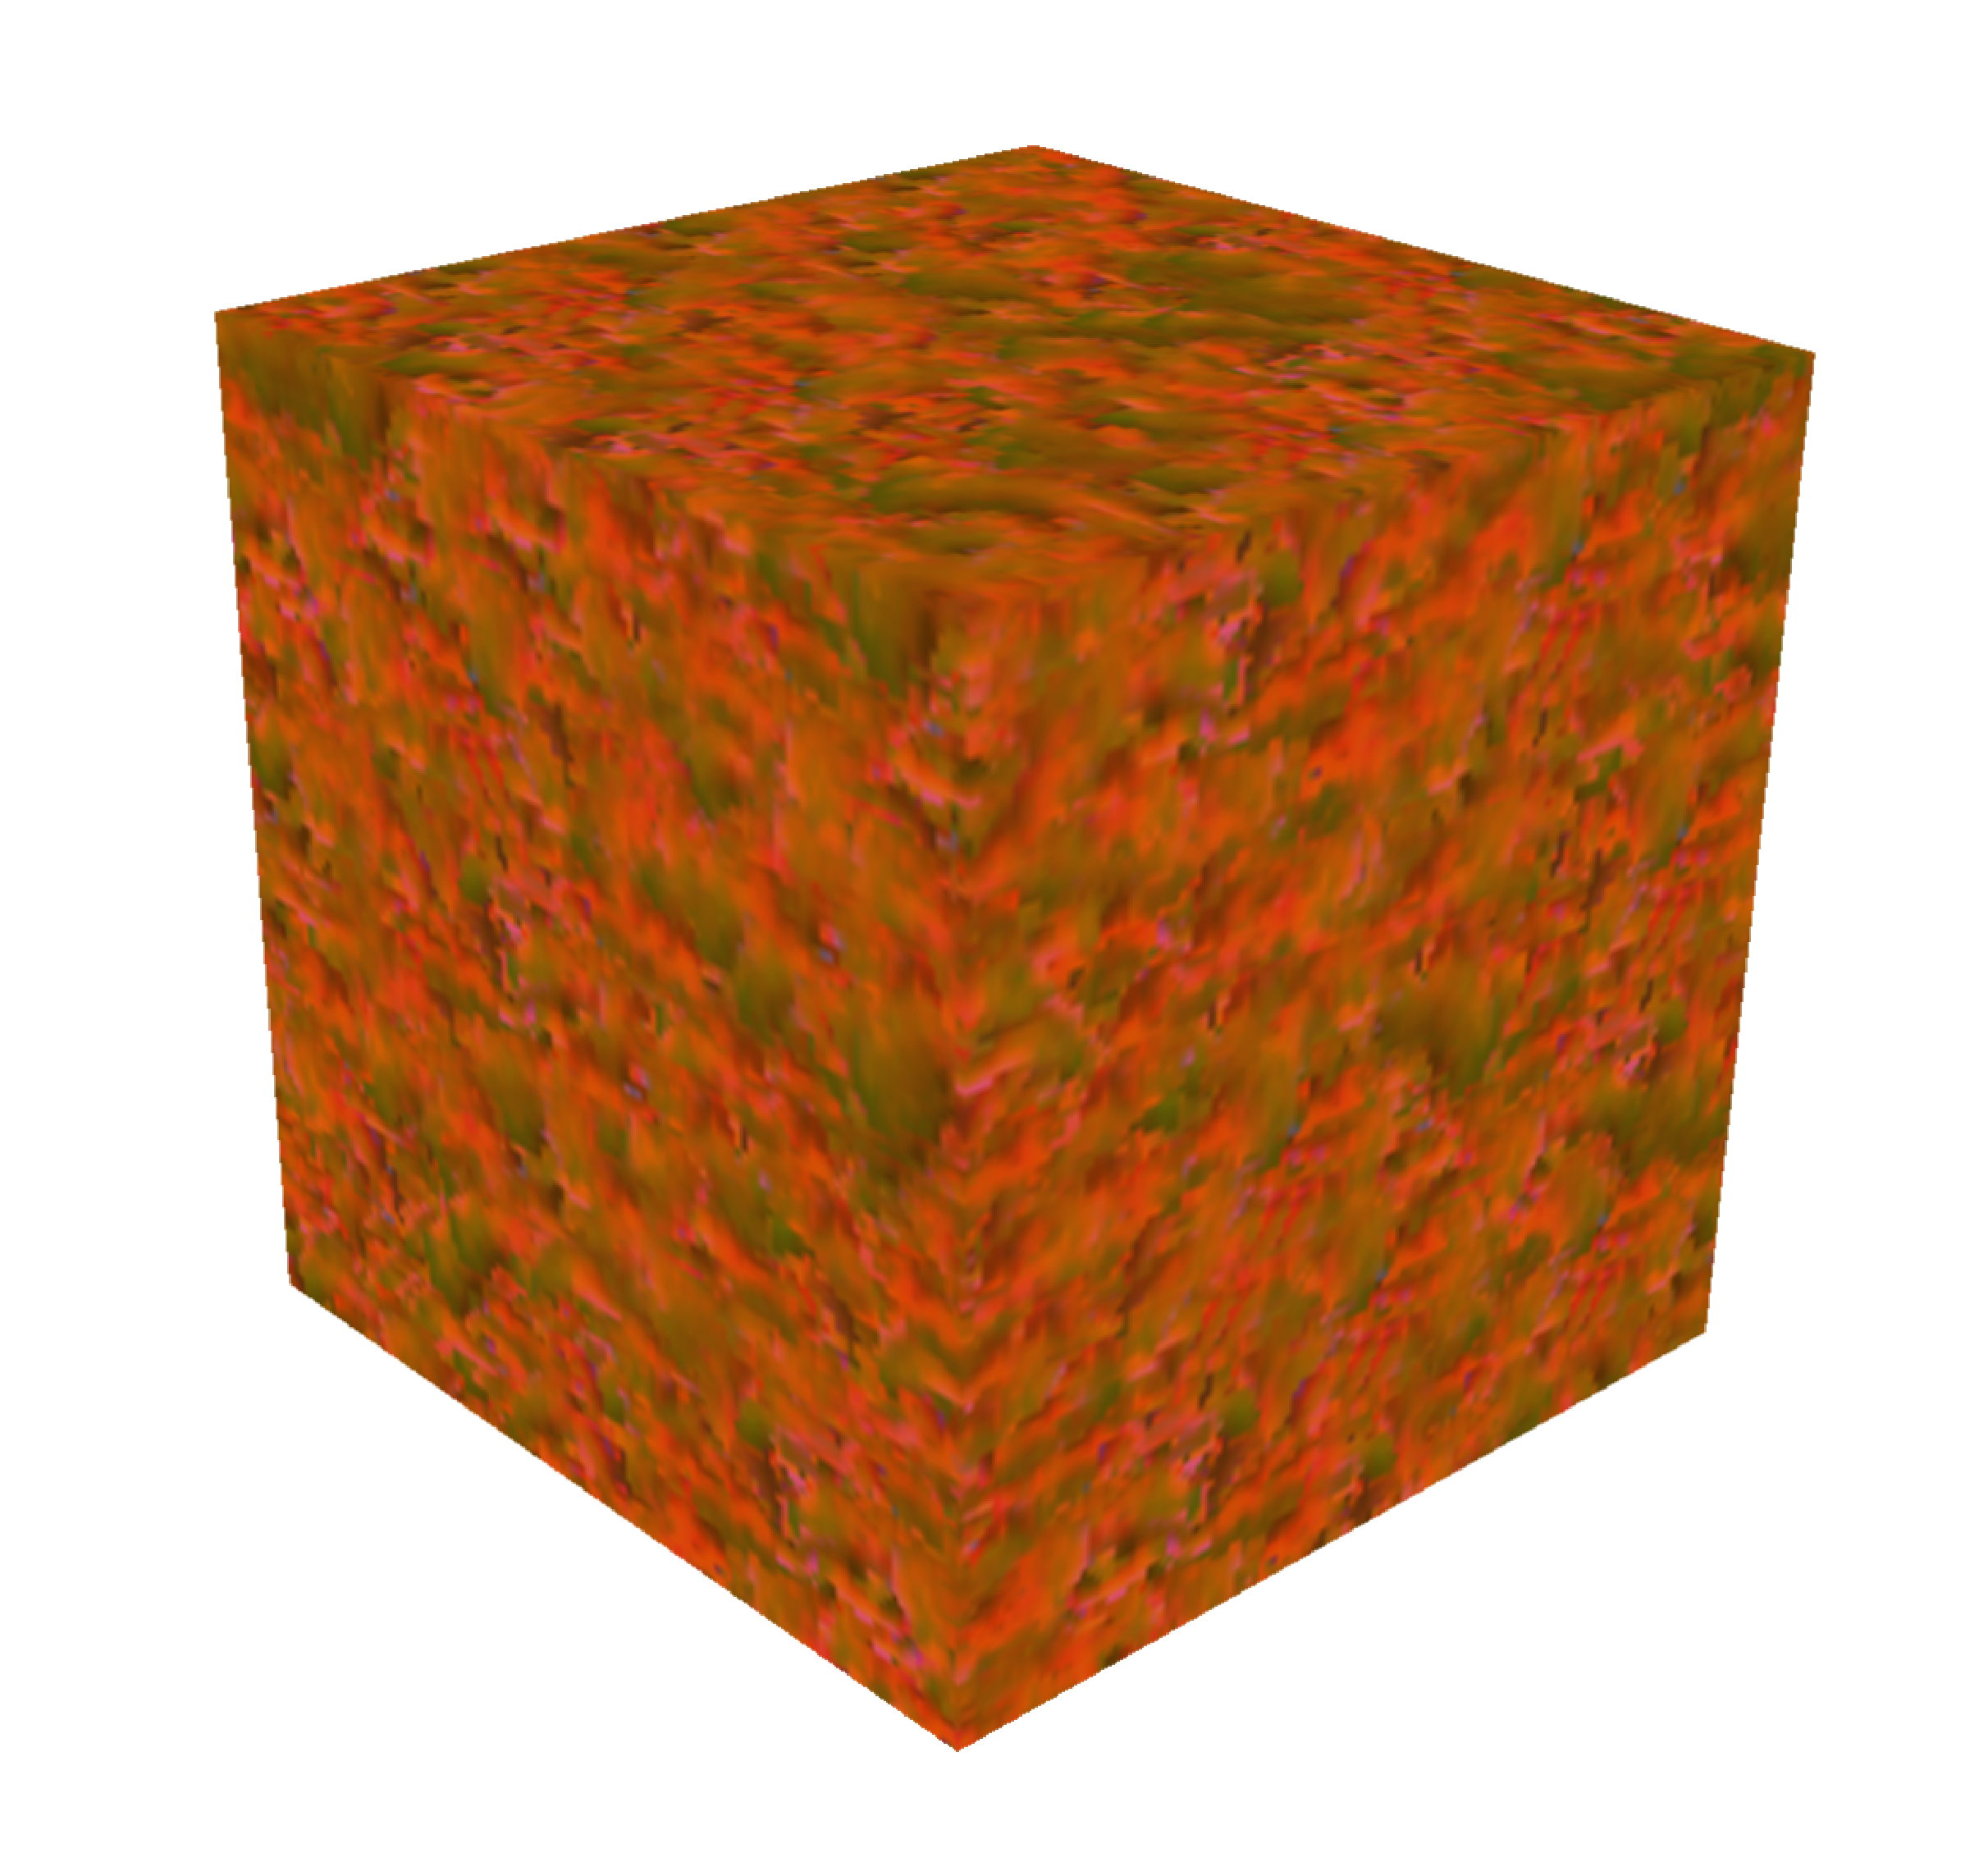
\epsfig{file = Left_HippocampusPhysicalParamsVolume.eps, width = 5cm}
	    }
 \subfigure[Amygdala's physical parameters]{
	    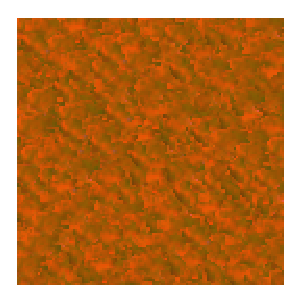
\epsfig{file = Left_AmygdalaSample.eps, width = 2cm}
	    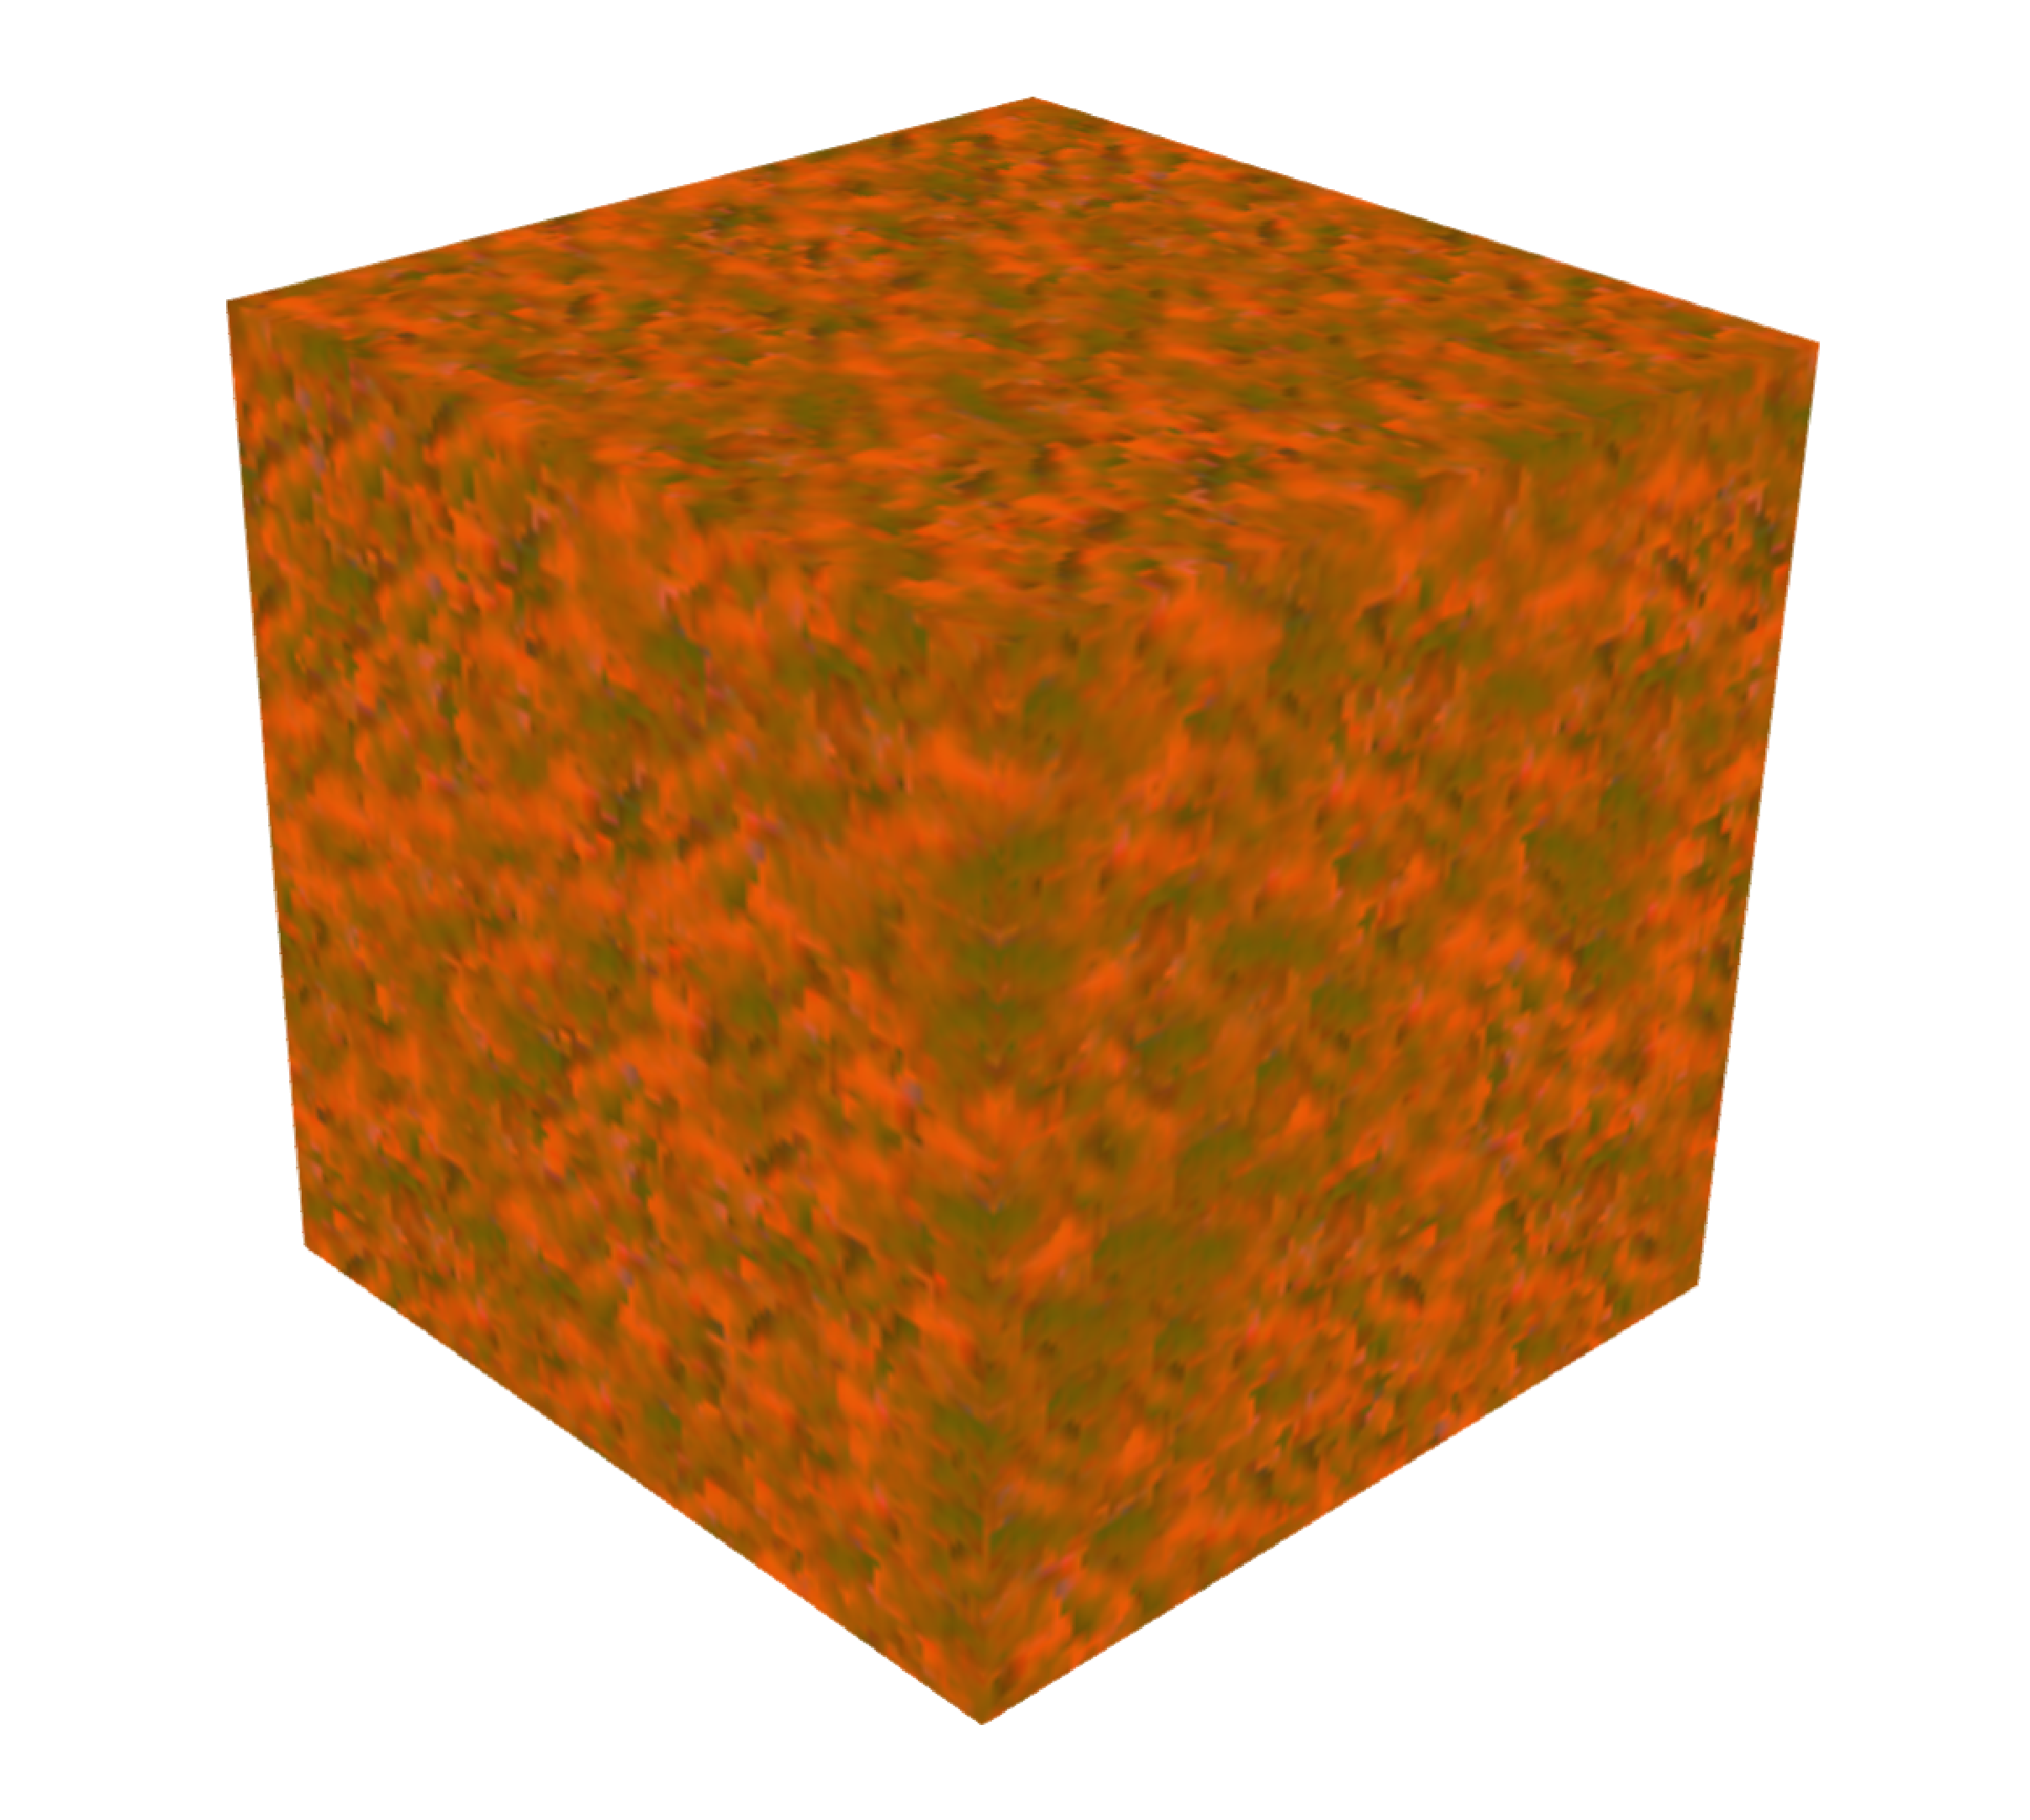
\epsfig{file = Left_AmygdalaSampleVolume.eps, width = 5cm}
	    } 
 \caption[Isotropic texture synthesis of physical parameters.]{Results of isotropic texture synthesis using images of physical parameters
          of the hippocampus (left) and amygdala (right). The images have been rescaled to [0-255].}
 \label{fig:isotropicsynthesisPhysical} 
\end{figure}

Figure \ref{fig:isotropicsynthesisPhysical} shows two synthesized volumes of physical parameters. 
The MRI values (see Chapter \ref{chapter:MRISimulation}) for each component are between the following intervals: 
$T_1 = [1672 - 4111]$ , $T_2 = [787 - 1793]$, $T_2^* = [54 - 2246]$ and $M0 = [20 - 595]$.
All of them are rescaled to $[0, 255]$ and are assigned red, green, blue and transparency respectively, this is done for visualization purposes.

The following sections shows the different type of textures that can be synthesized by the approach.

\subsection{Anisotropic texture from many 2D exemplar textures}

\begin{figure}[h!] 
 \centering 
 \subfigure[Exemplar textures.]{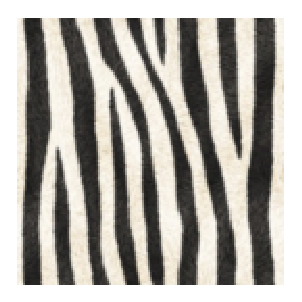
\epsfig{file = zebra.eps, width = 2cm}
	    
\epsfig{file = zebraAx.eps, width = 2cm}
	   }
 \subfigure[Generated volume.]{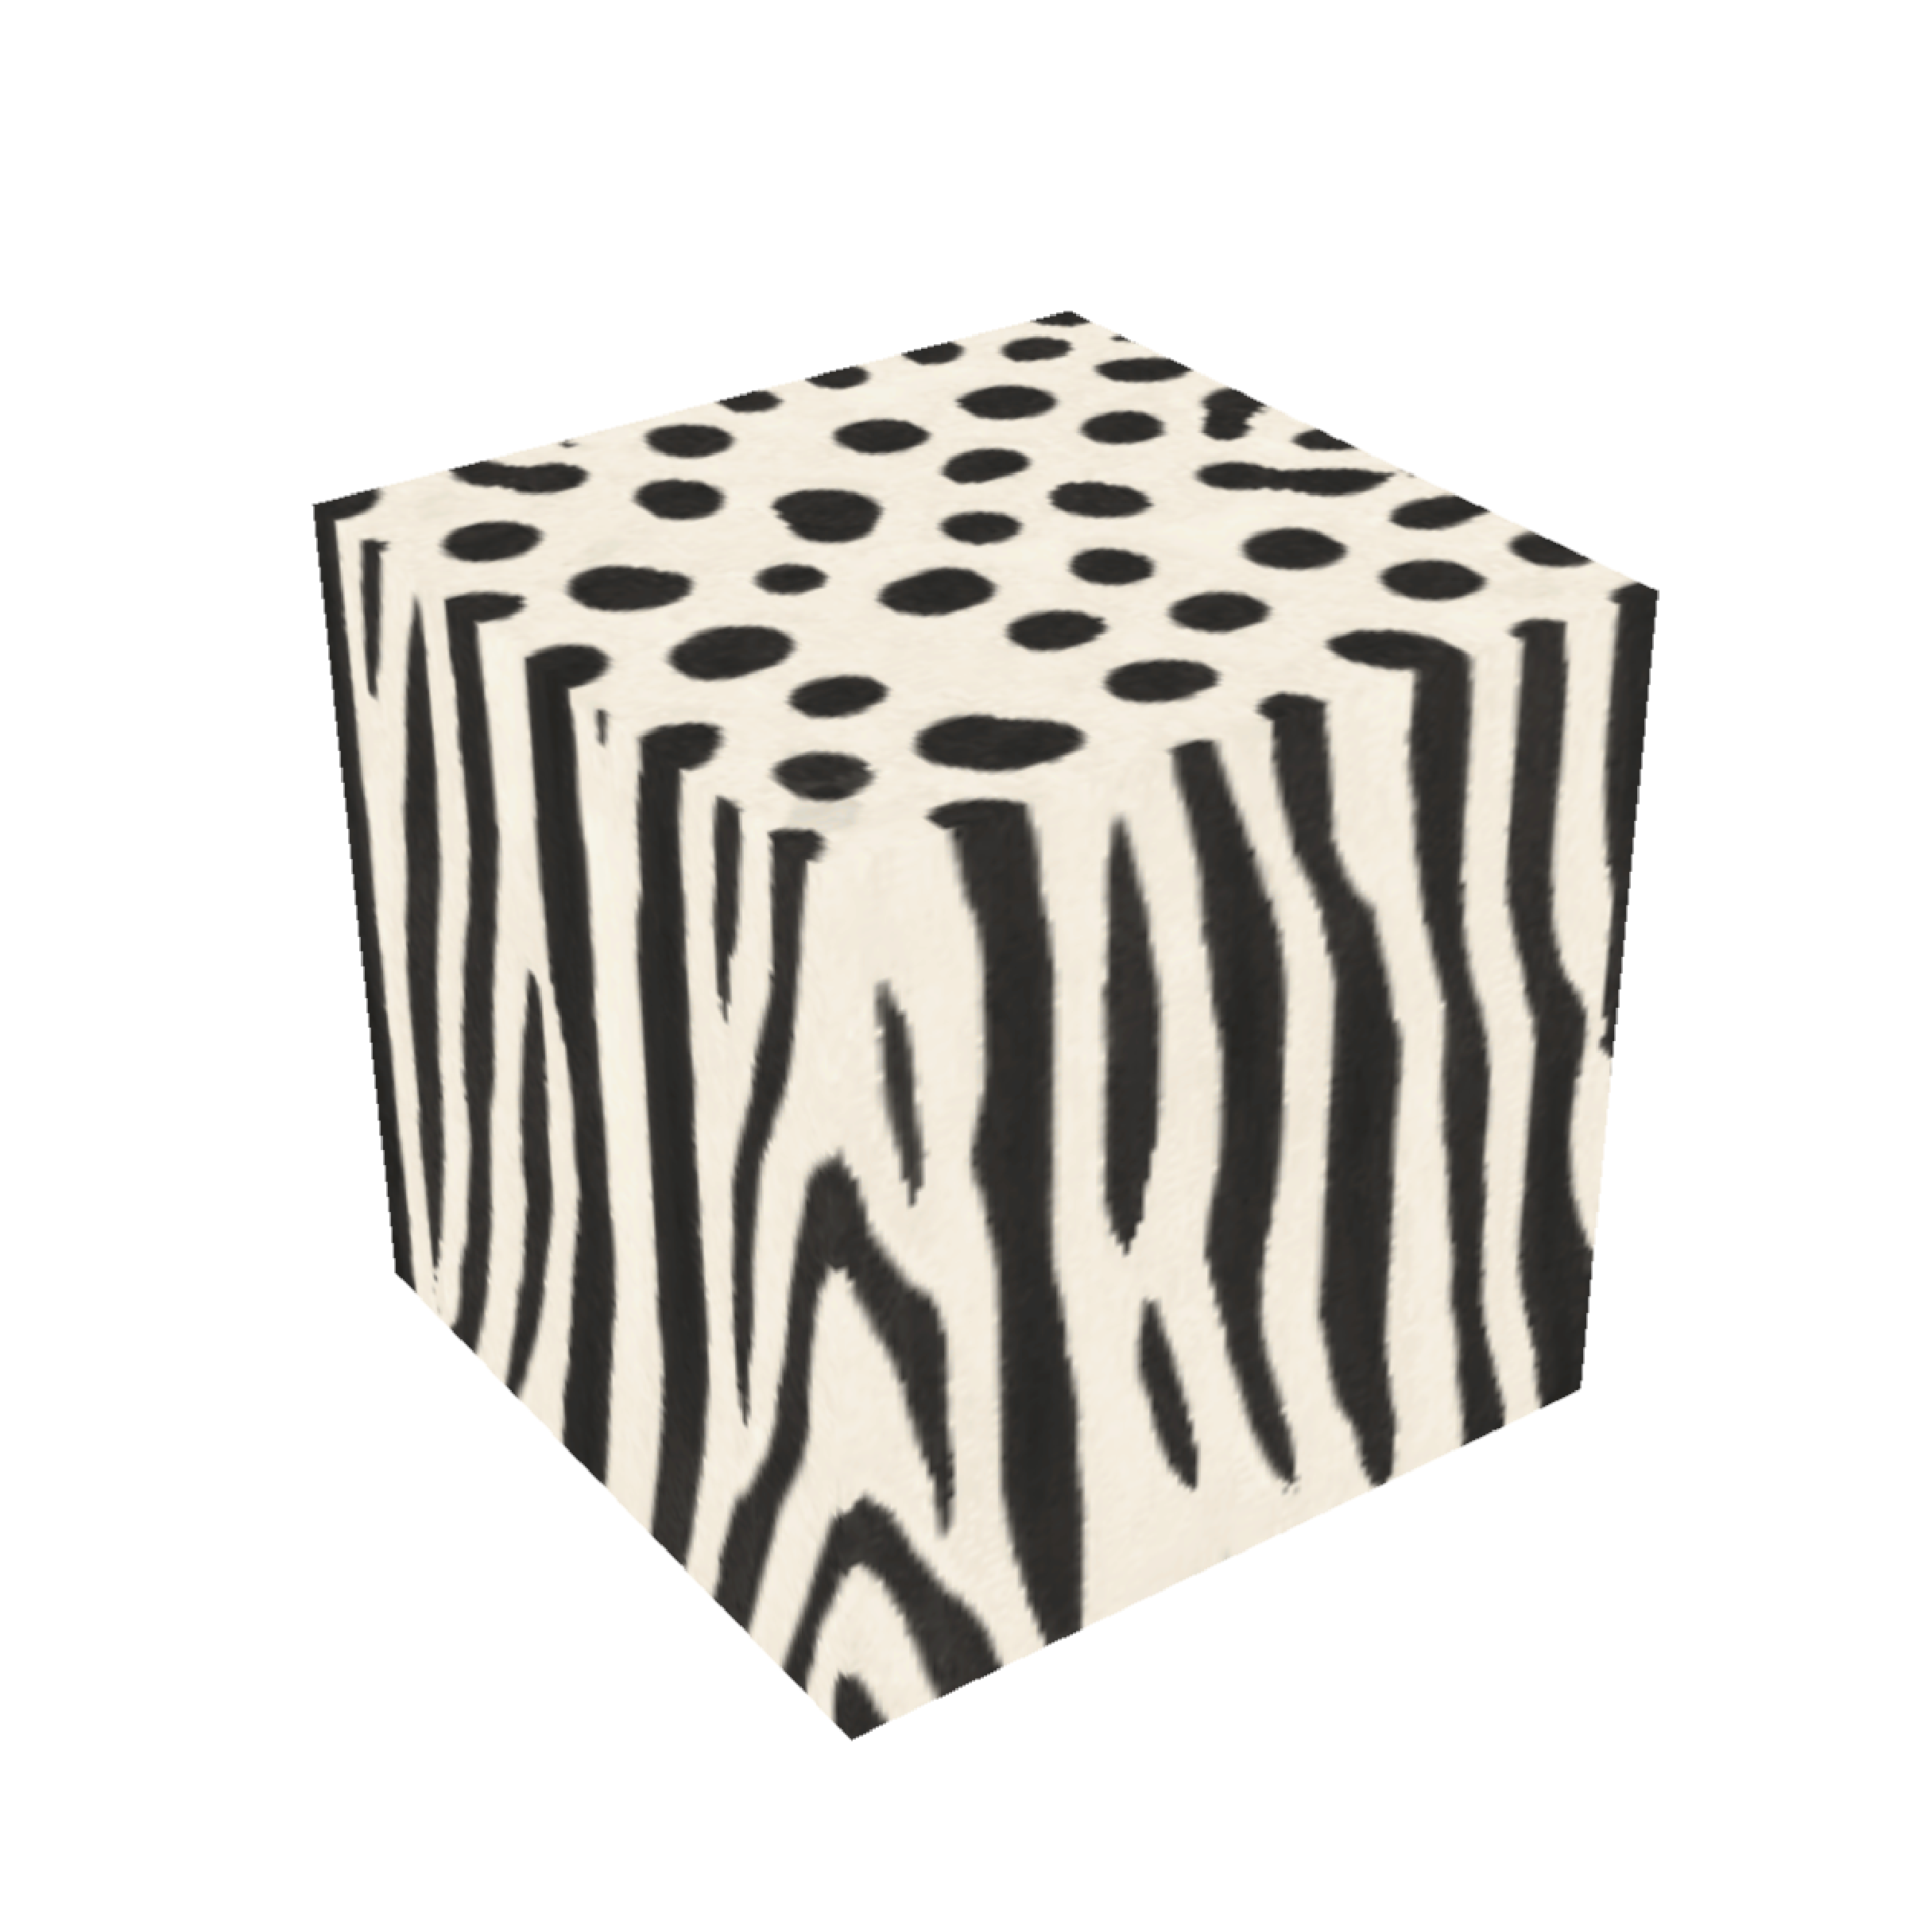
\epsfig{file = zebraVol.eps, width = 5cm}}
 \subfigure[Surface rendering.]{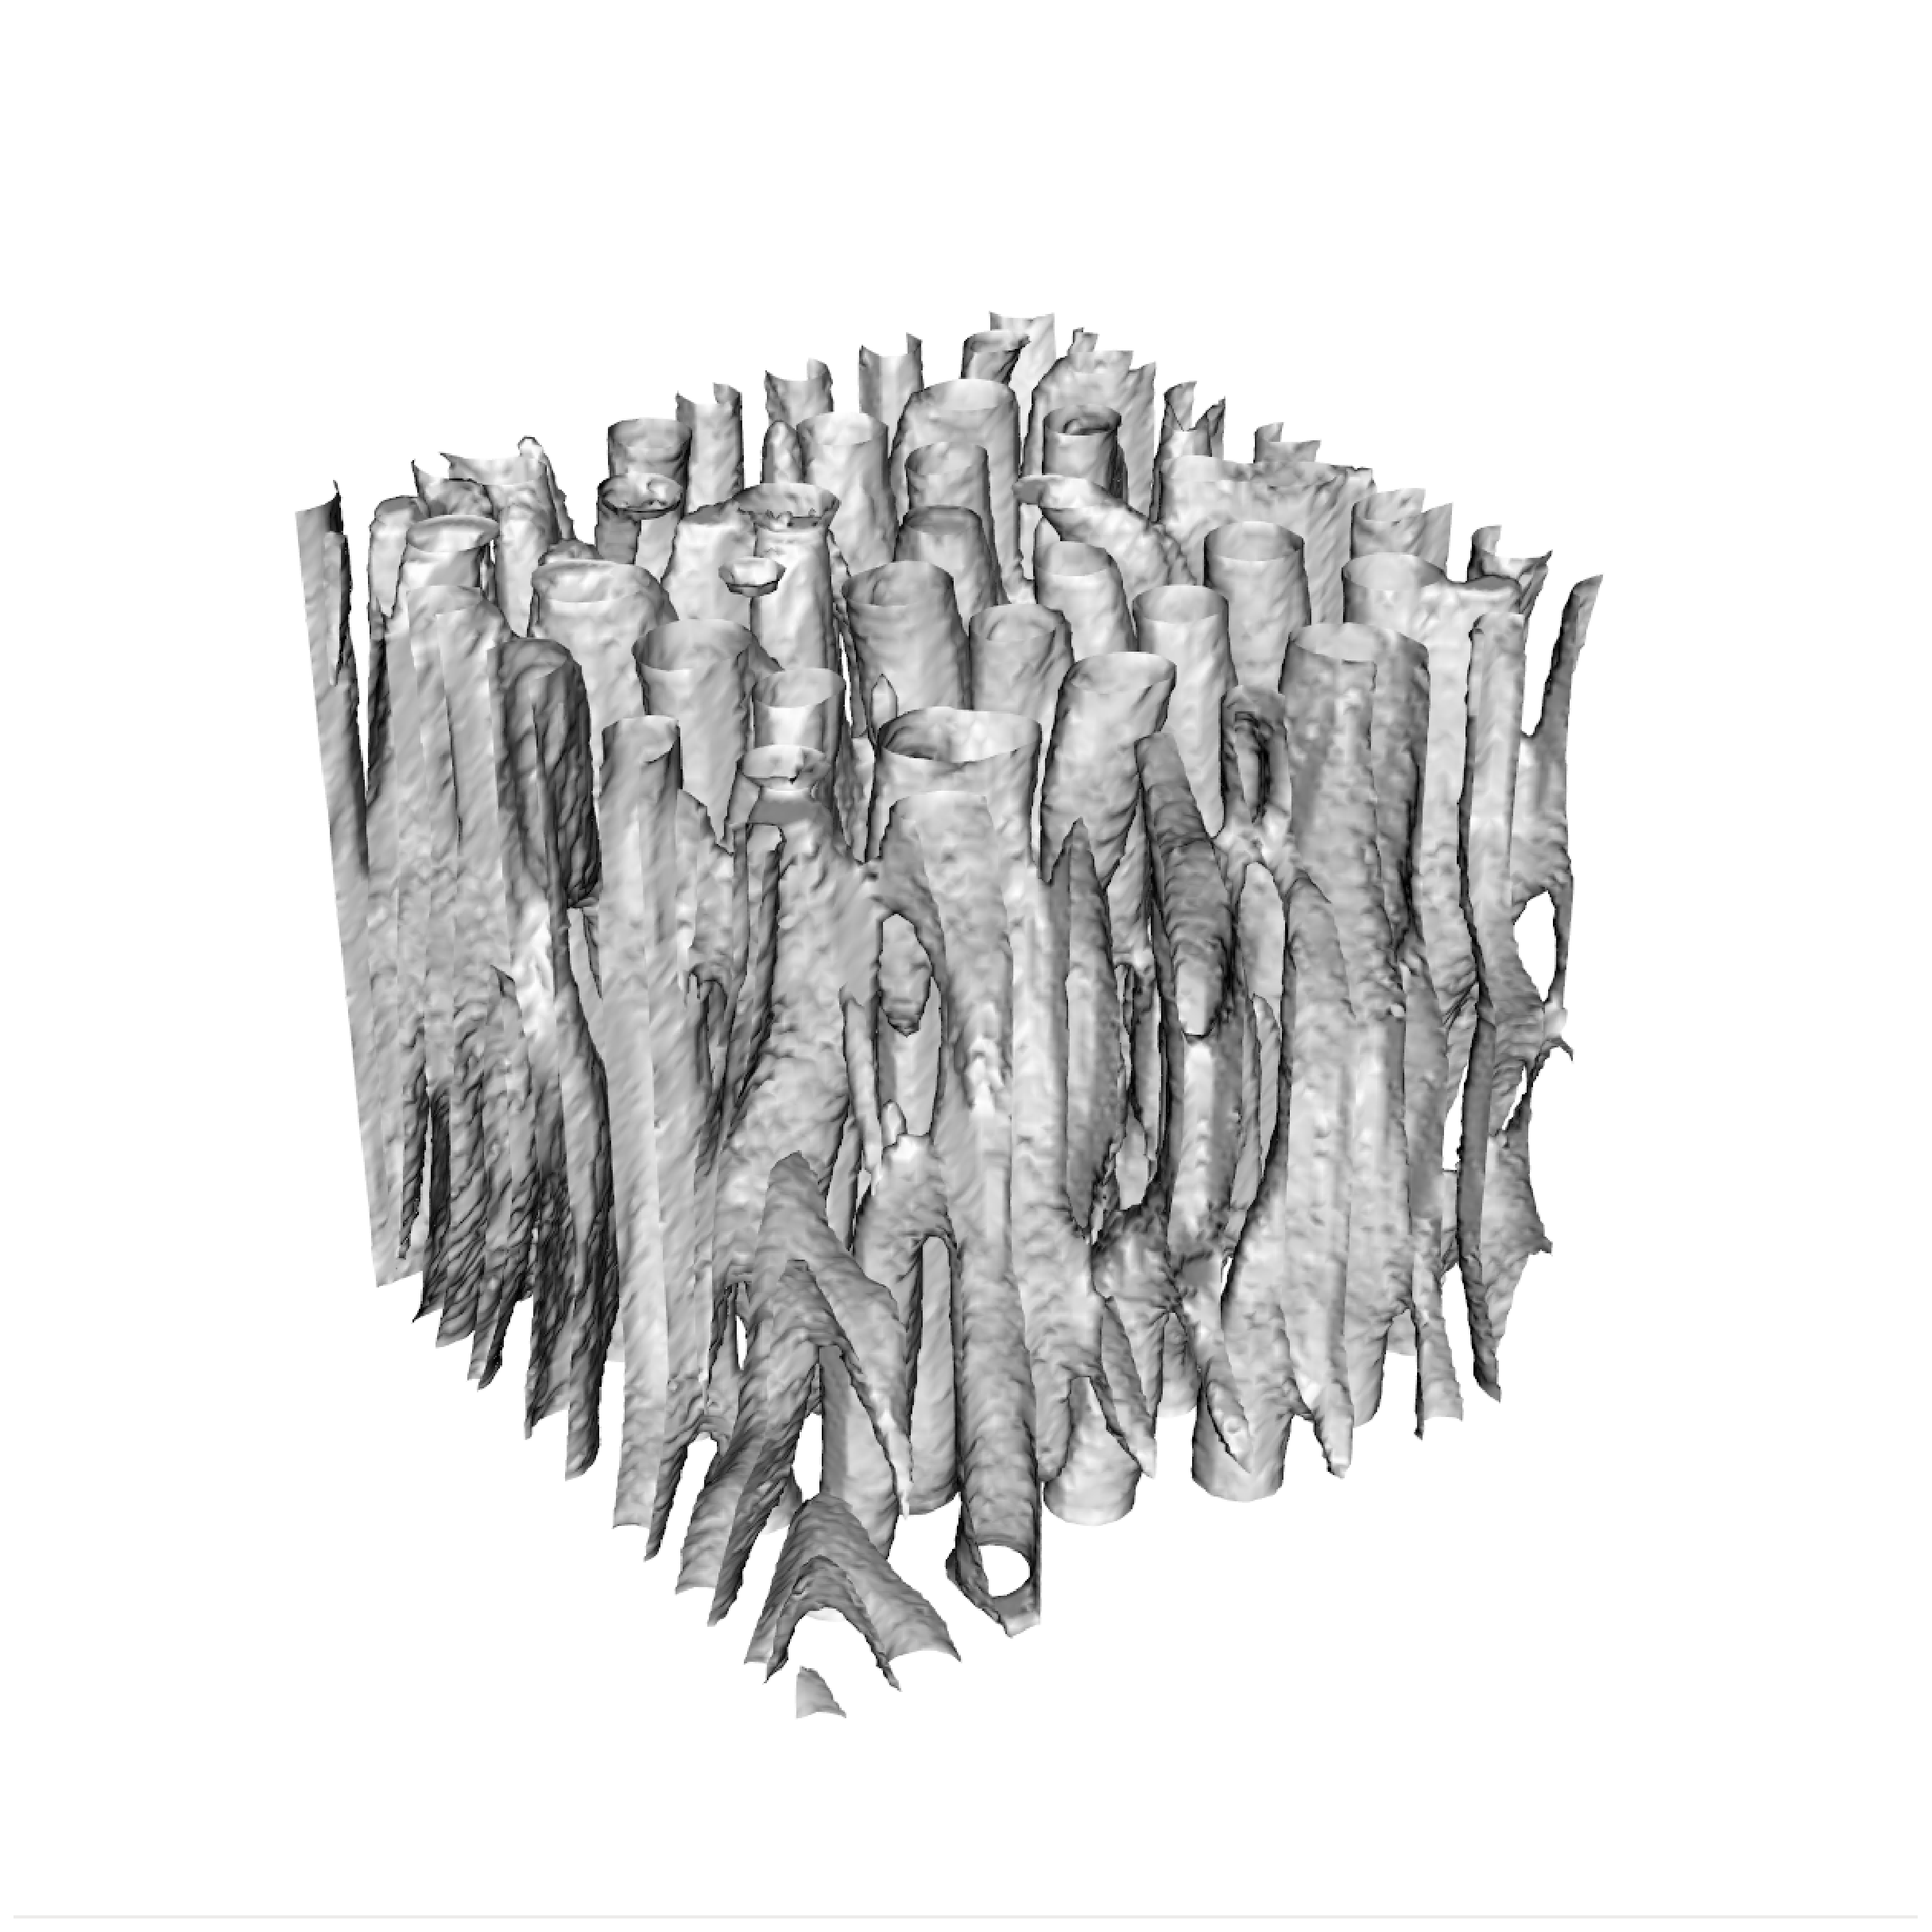
\epsfig{file = zebraSurf.eps, width = 5cm}}
 \caption[Anisotropic texture synthesis.]{Results of anisotropic synthesis. The optimization was performed using the zebra texture to constraint the longitudinal and transversal planes. The dot texture was used in the axial plane.}
 \label{fig:3DAnisotropicTexture} 
\end{figure}

Many anatomical structures and materials 
have different orientations and scales. 
These features can be illustrated by creating a texture that mimics these variations. 

Figure \ref{fig:3DAnisotropicTexture} shows the result of selecting two different textures 
to constrain the optimization.
Selecting the zebra texture and the dot pattern generated cylinder like structures. 
This is done by doing the search phase for the longitudinal and transversal planes in the zebra texture, 
while the axial plane does the search phase in the dot texture.
 
When rendering the surface of the object, we can see that the generated structure 
is very complex and consists of tubes that join and separate at arbitrary slices.
This synthetic structure can be used to test Brownian simulation algorithms 
that reveal the environment's structures.

\subsection{Anisotropic texture constrained by additional masks }

\begin{figure}[h!]
 \centering 
 \subfigure[Exemplar textures + binary masks.]{
\epsfig{file = myocyte.eps, width = 2cm}
	    
\epsfig{file = myocyteSgMask.eps, width = 2cm} \hspace{1cm}
	    
\epsfig{file = myocyteAx.eps, width = 2cm}
	    
\epsfig{file = myocyteAxMask.eps, width = 2cm}
	   } \\
 \subfigure[Longitudinal view of the volume.]{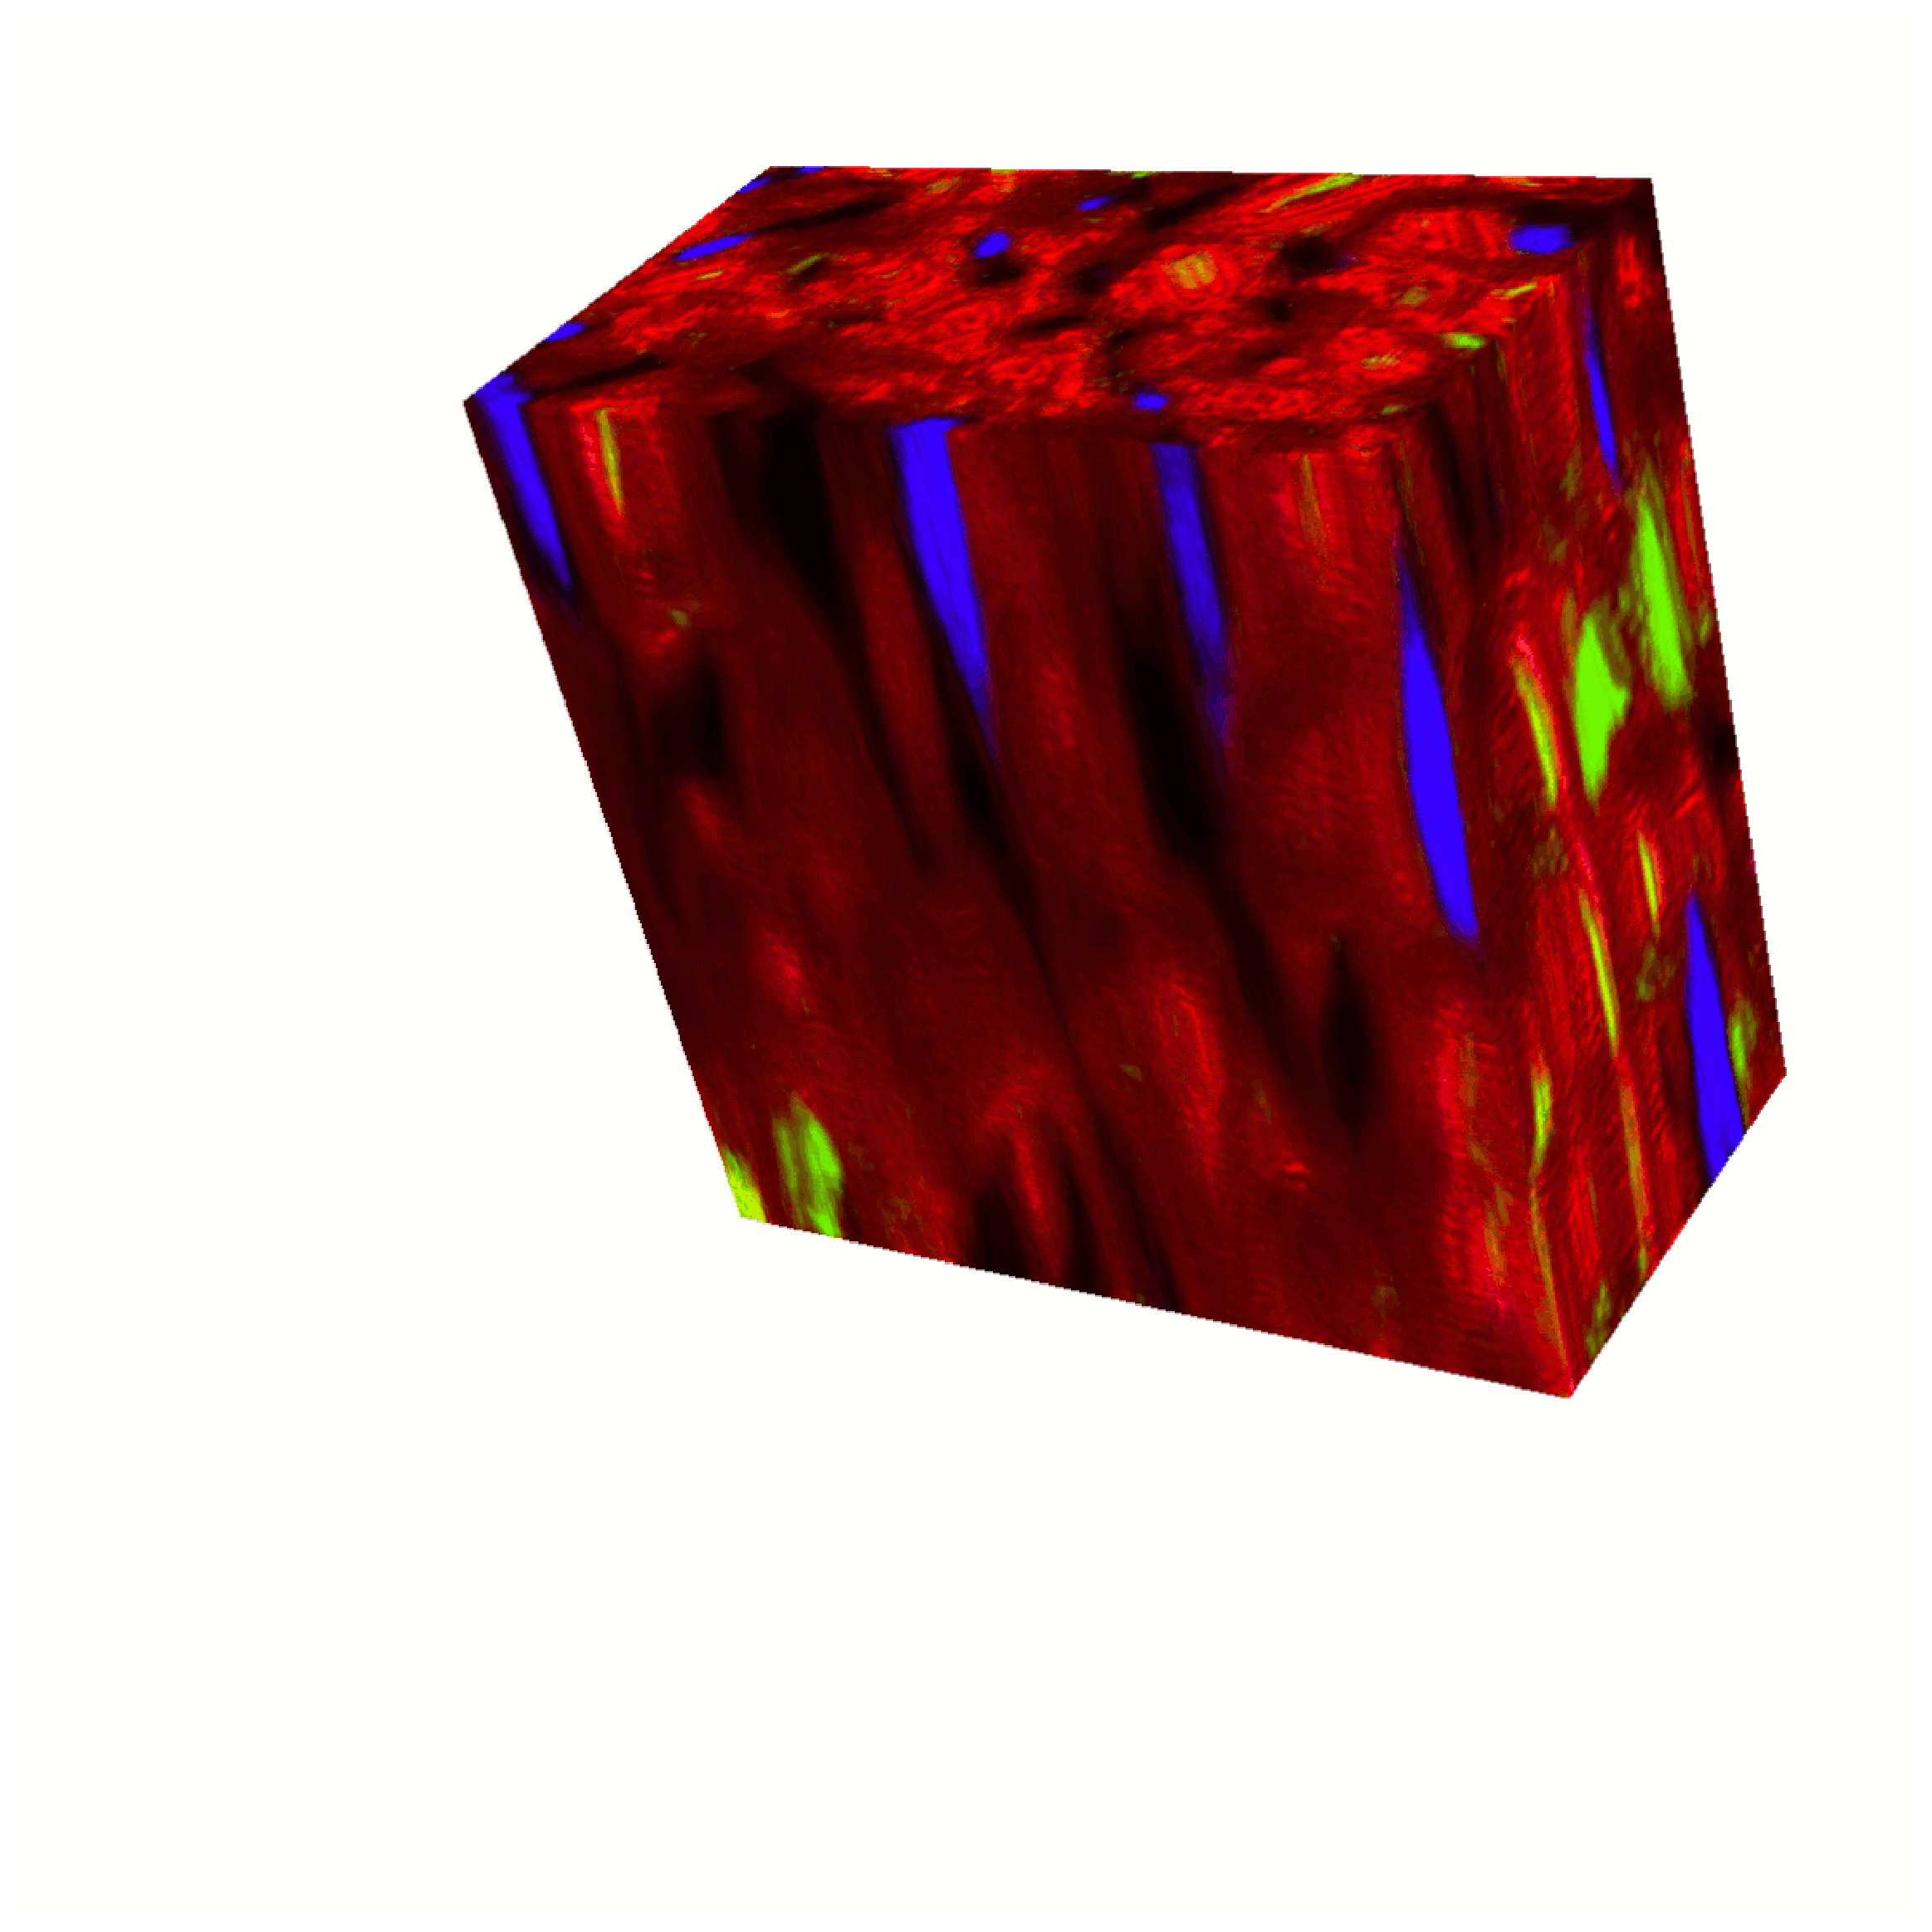
\epsfig{file = myocyteSgVol.eps, width = 5cm}}
 \subfigure[Axial view of the volume]{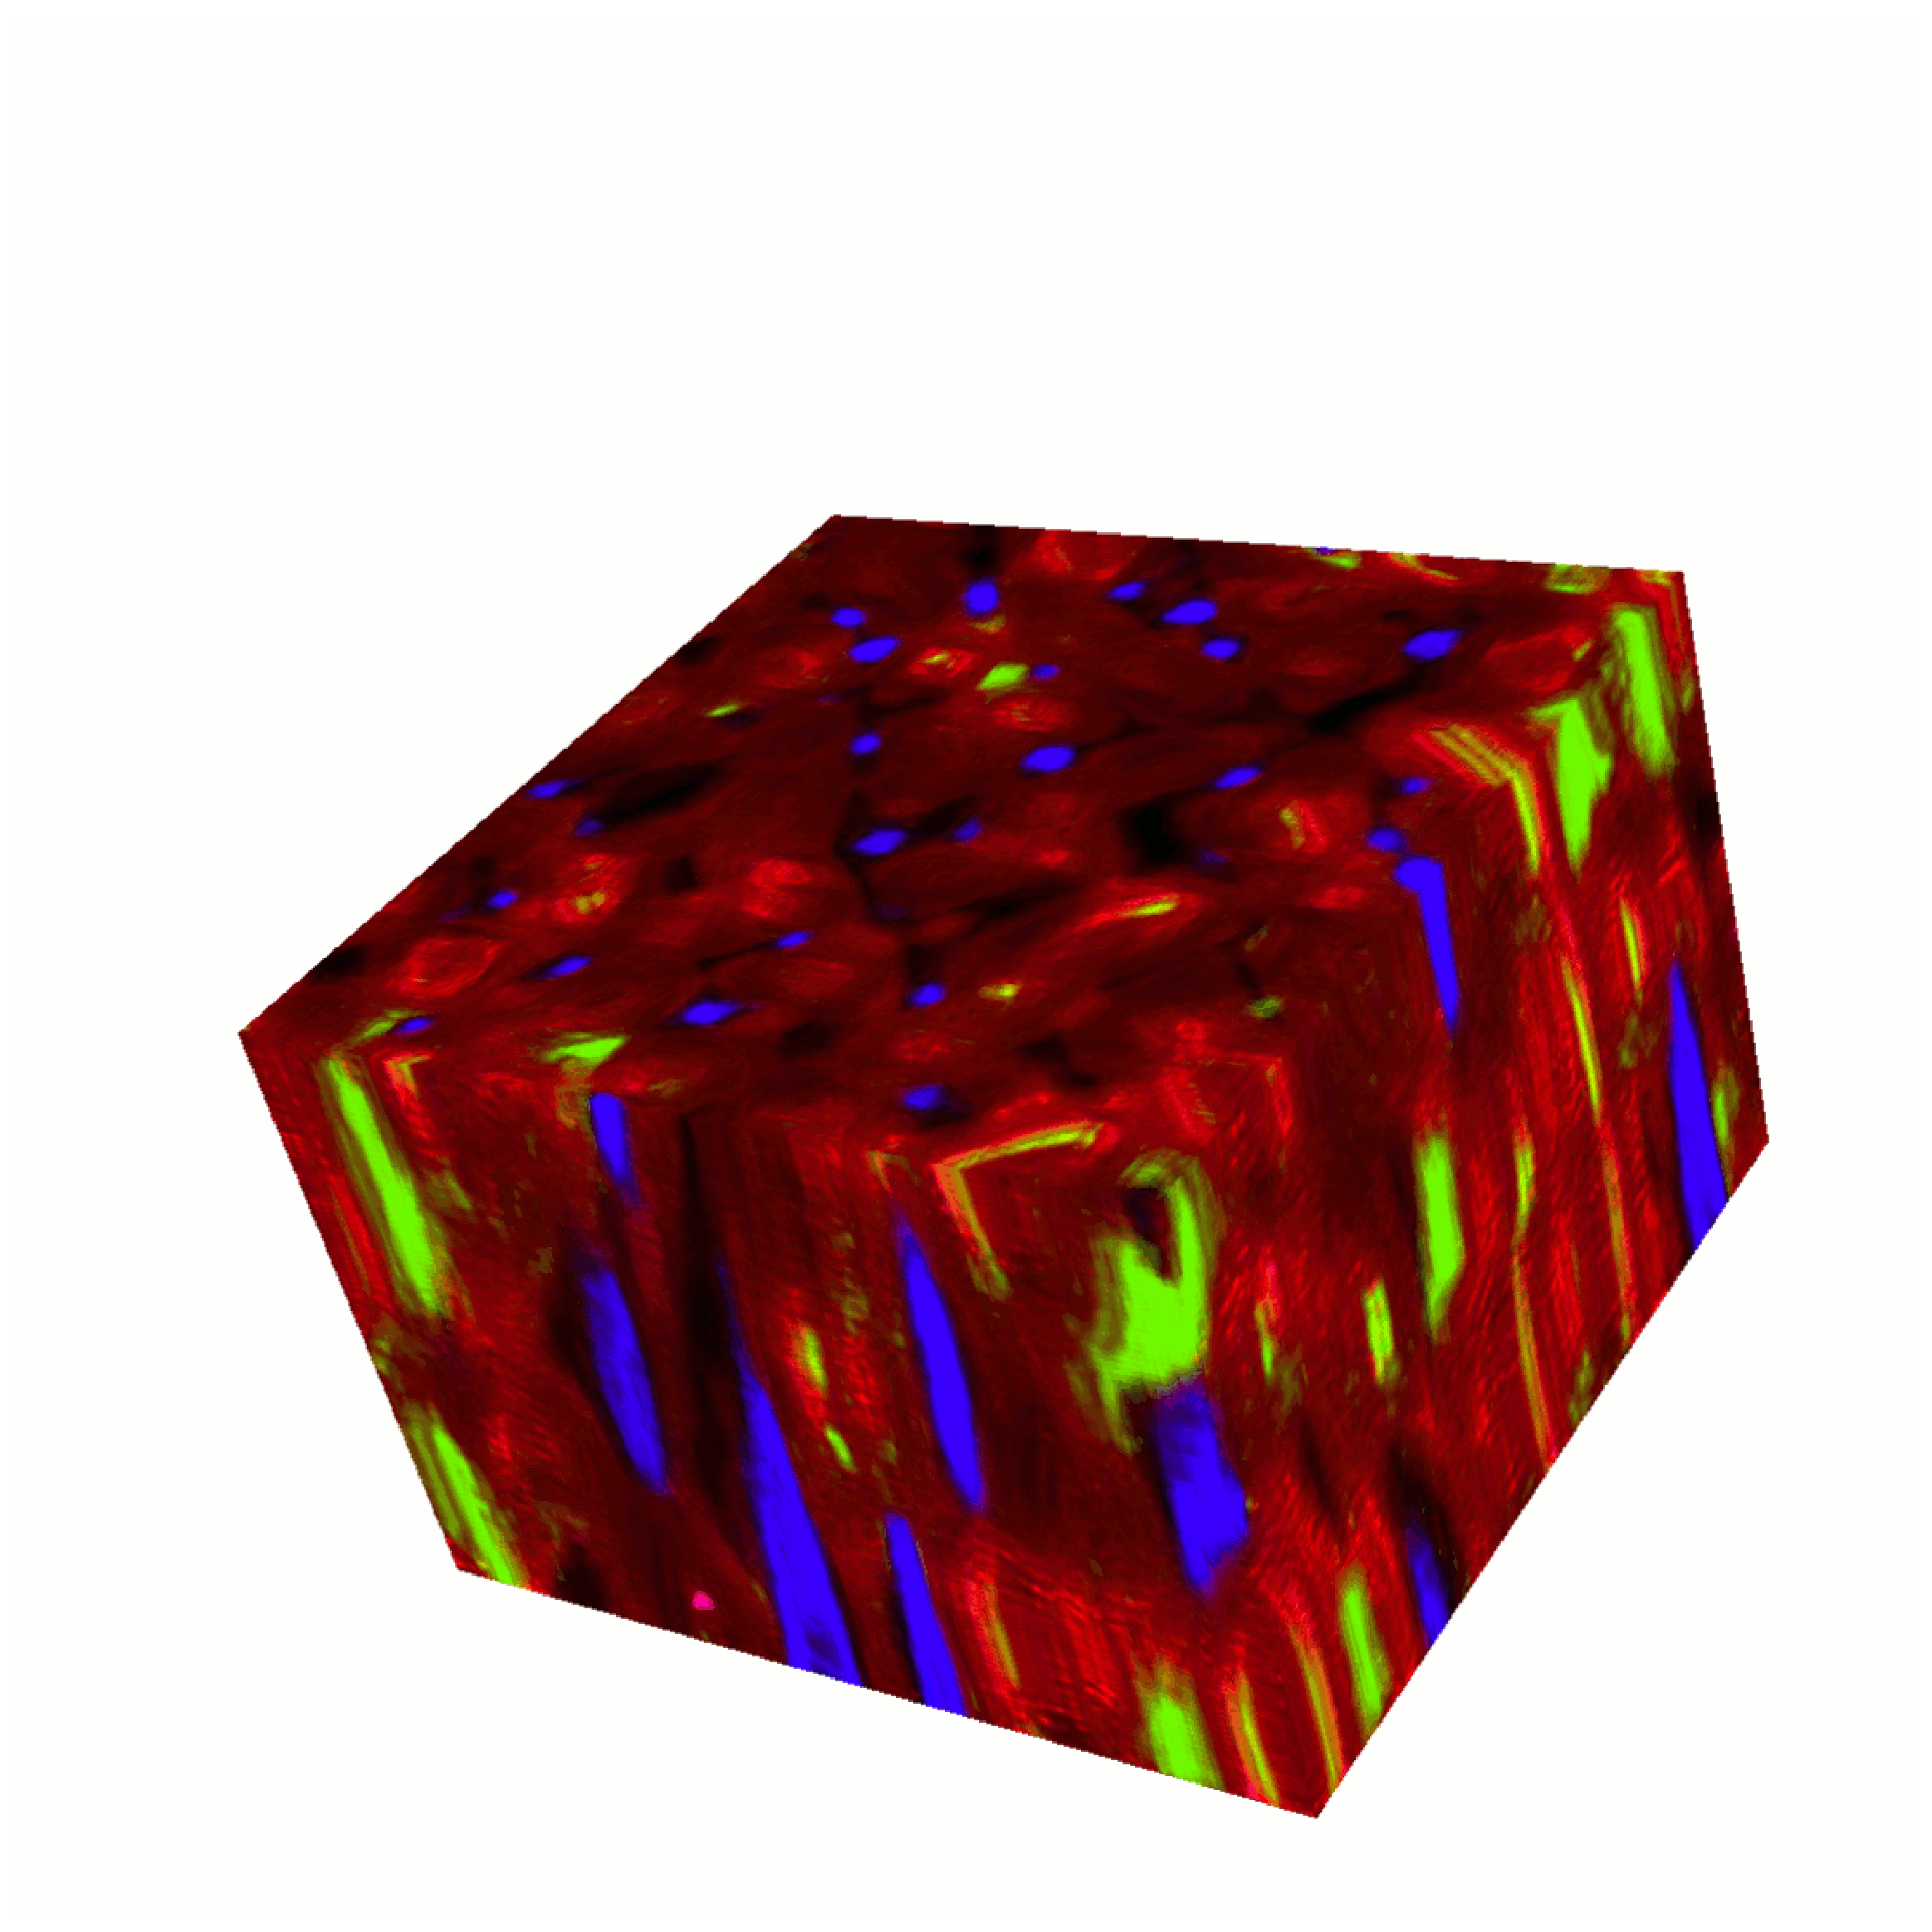
\epsfig{file = myocyteAxVol.eps, width = 5cm}
				  }
 \caption[Anisotropic texture synthesis and distance maps.]{Results of anisotropic synthesis starting from two different textures and their additional binary masks.}
 \label{fig:3DAnisotropicTextureAndMask}
\end{figure}

It is possible to use a distance map as an extra channel, in addition to the RGB components.
A binary image of the texture can be used to compute a distance map.
This is useful when the texture has large unstructured areas \cite{Lefebvre:2006:ATS:1141911.1141921}.

Figure \ref{fig:3DAnisotropicTextureAndMask} shows the synthesis results using different exemplar textures obtained from confocal 
images\footnote{\url{http://www1.ic.ac.uk/medicine/people/p.camelliti/}} and the corresponding binary masks. 
A signed Euclidean distance map is computed from the binary image and used as an extra channel in the synthesis procedure.

The 3D texture representing a myocyte cell tissue are quite representative of tissue viewed as complexes of cells (myocytes in red and fibroblasts in blue).
The anisotropy of the cells is conspicuous and the contrast of staining is well preserved thanks to the use of the binary masks. 
%The 3D texture represents a myocyte cell tissue.

One main advantage of this method is to generate a 3D tissue from 2D information. 
Up to now, it was impossible for the biologist or the physician to have a 3D representation 
of the cell tissue, since it is technically very difficult or even impossible to have 
an axial resolution as good as those in the slice. 
Thanks to this approach, the experts can get a virtual 3D representation of the tissues 
that are close to reality.


\begin{figure}[h!] 
 \centering
 \subfigure[2D reference textures extracted from real images and binary masks.]{
 			\label{fig:ResultVolumes_exemplar}
%	    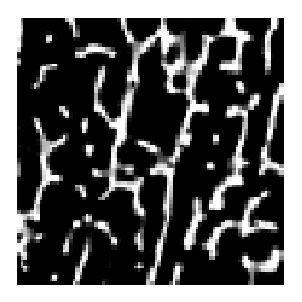
\epsfig{file = 42.irm_Y_015.eps, width = 1cm}
%	    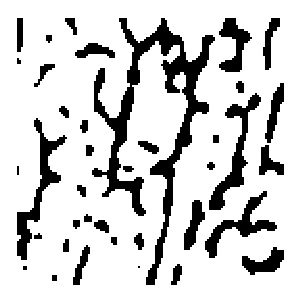
\epsfig{file = 42.irm_Y_015Mask.eps, width = 0.5cm}            
%	    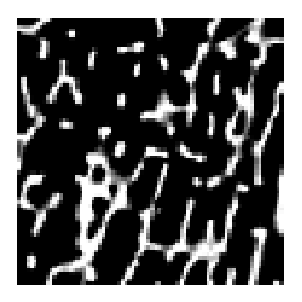
\epsfig{file = 42.irm_Y_047.eps, width = 1cm}
%	    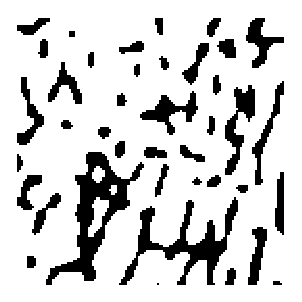
\epsfig{file = 42.irm_Y_047Mask.eps, width = 0.5cm}
%	    \hspace{0.5cm}
%	    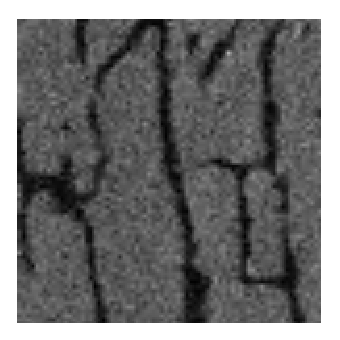
\epsfig{file = vol.73-93-94-sliceX.eps, width = 1cm}
%	    
\epsfig{file = vol.73-93-94-sliceXMask.eps, width = 0.5cm}                        
%	    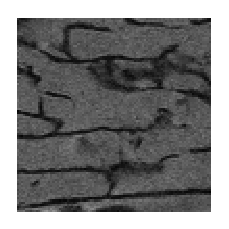
\epsfig{file = vol.73-93-94-sliceZ.eps, width = 1cm} 
%	    
\epsfig{file = vol.73-93-94-sliceZMask.eps, width = 0.5cm}}\\
% \subfigure[3D virtual images.]{
% 			\label{fig:ResultVolumes_textures}
% 			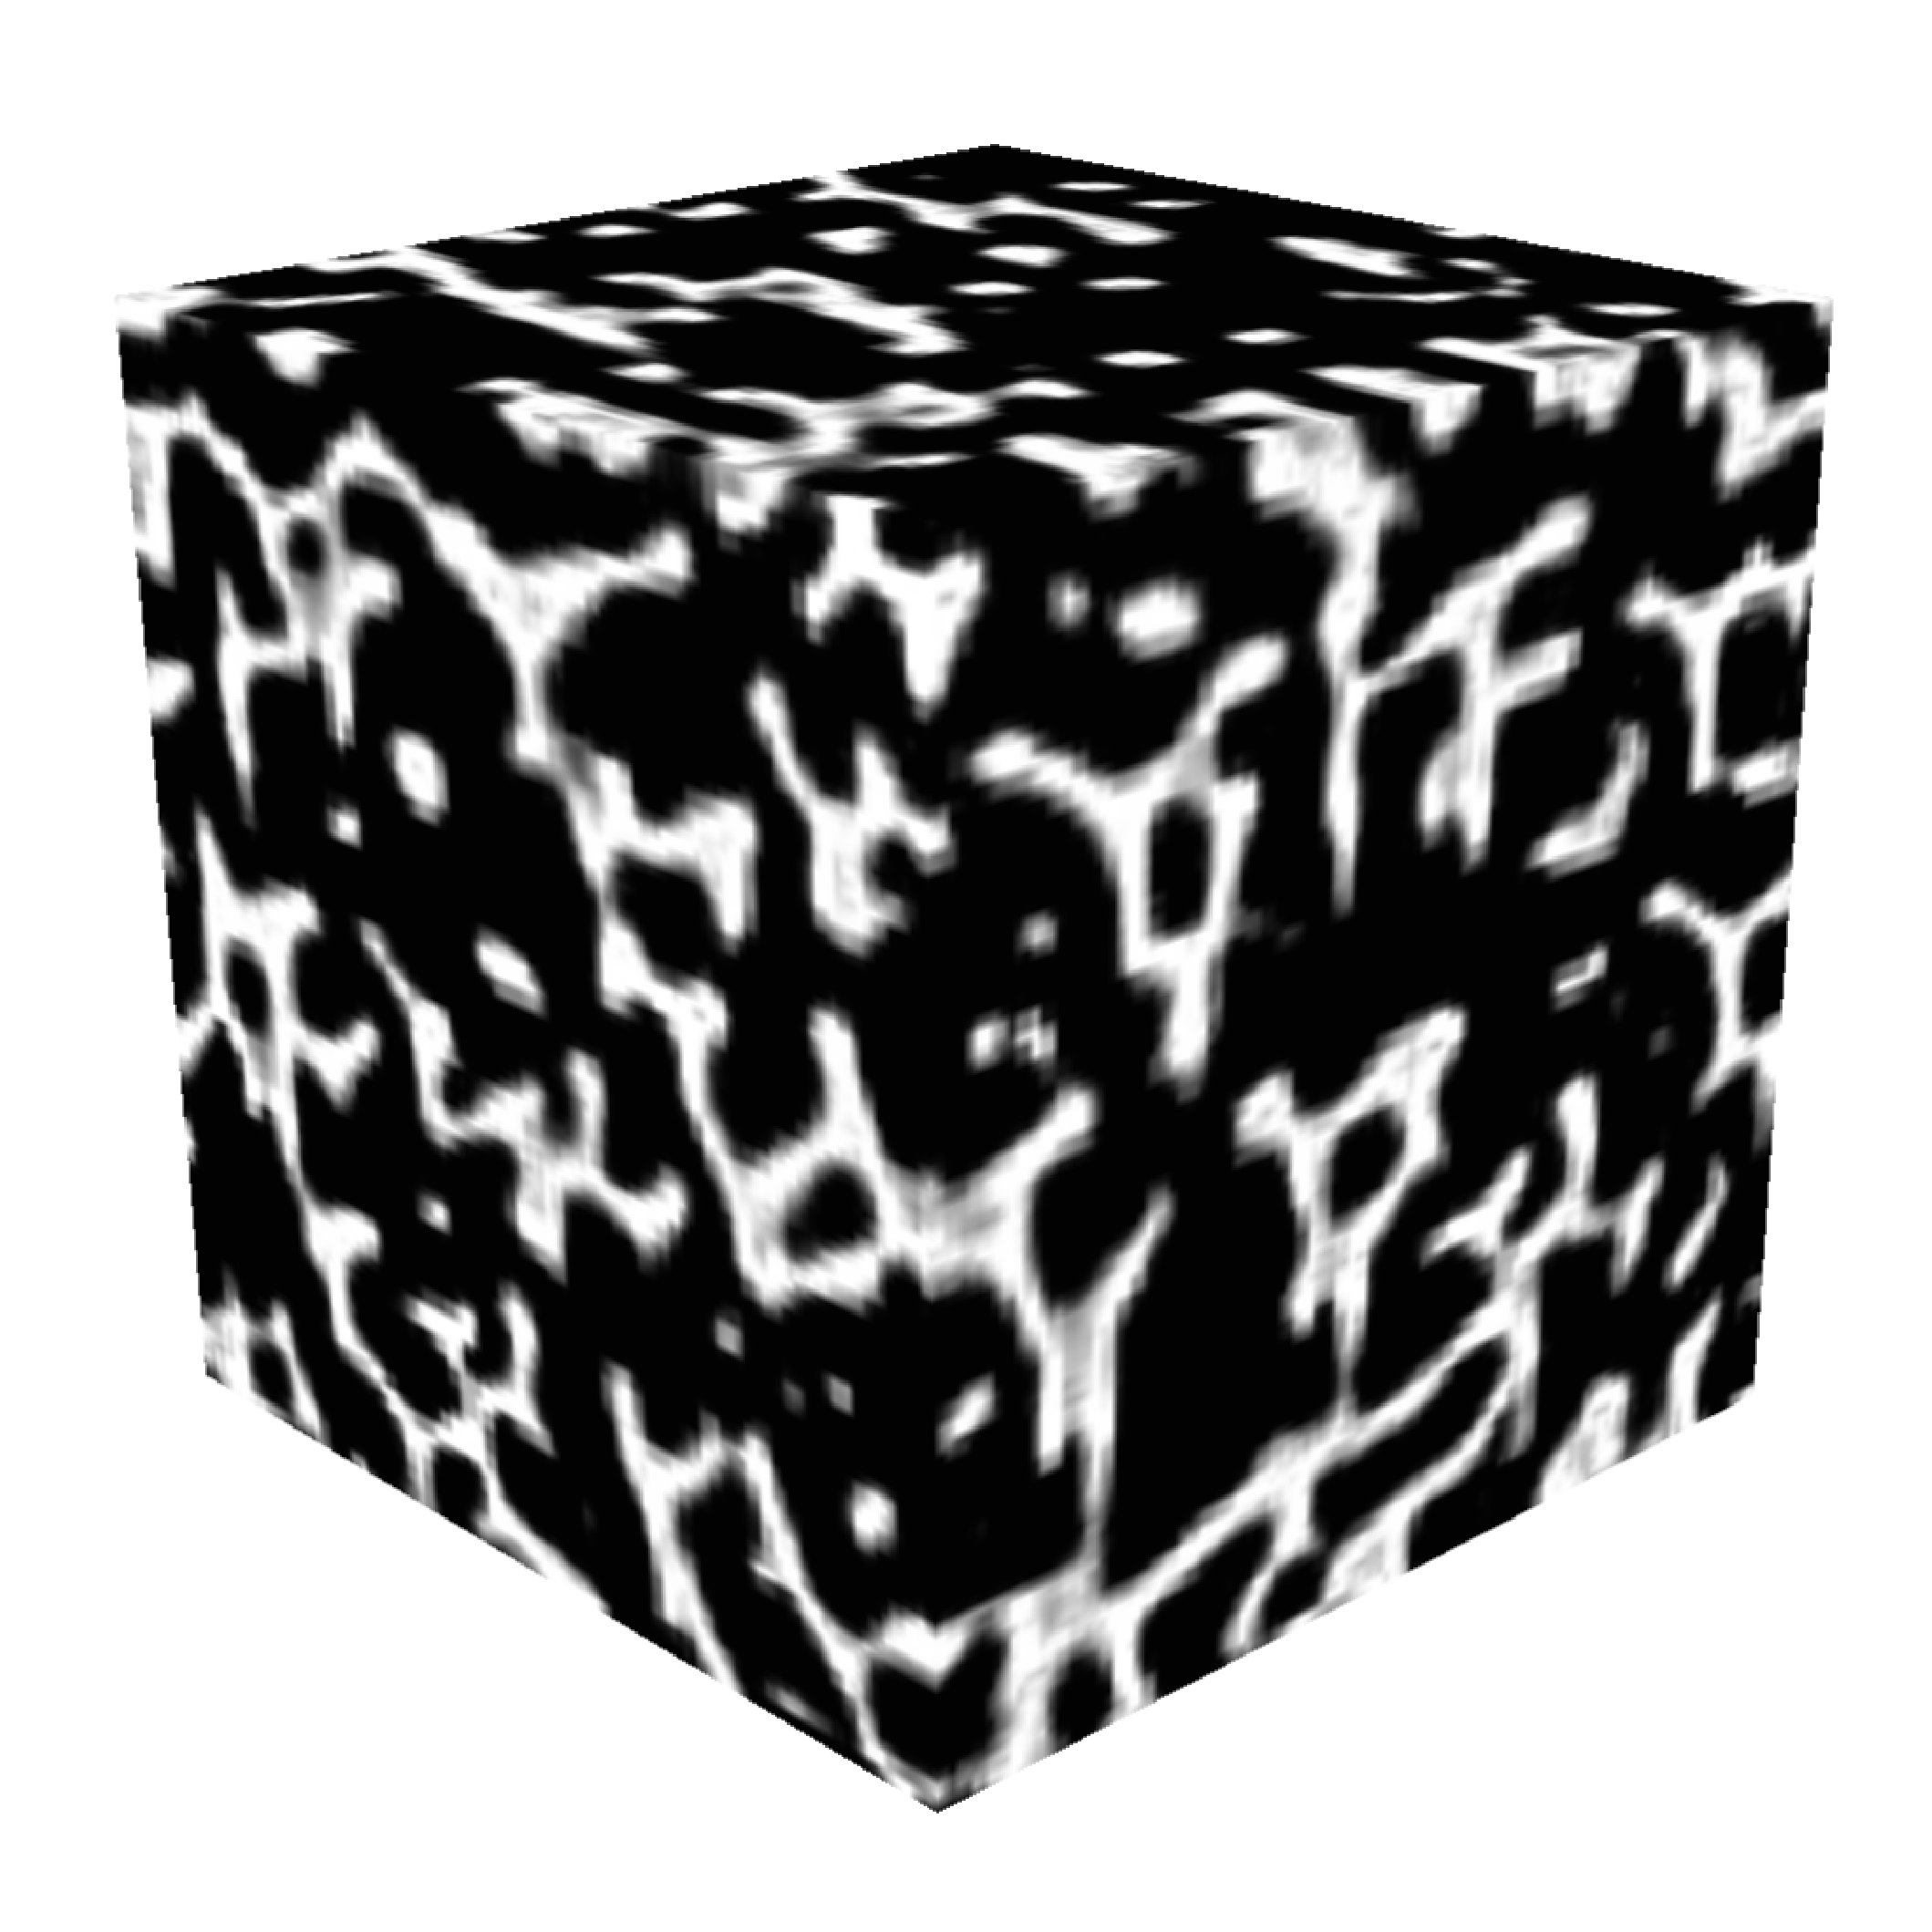
\epsfig{file = ModelESRF.eps, width = 3cm}
%			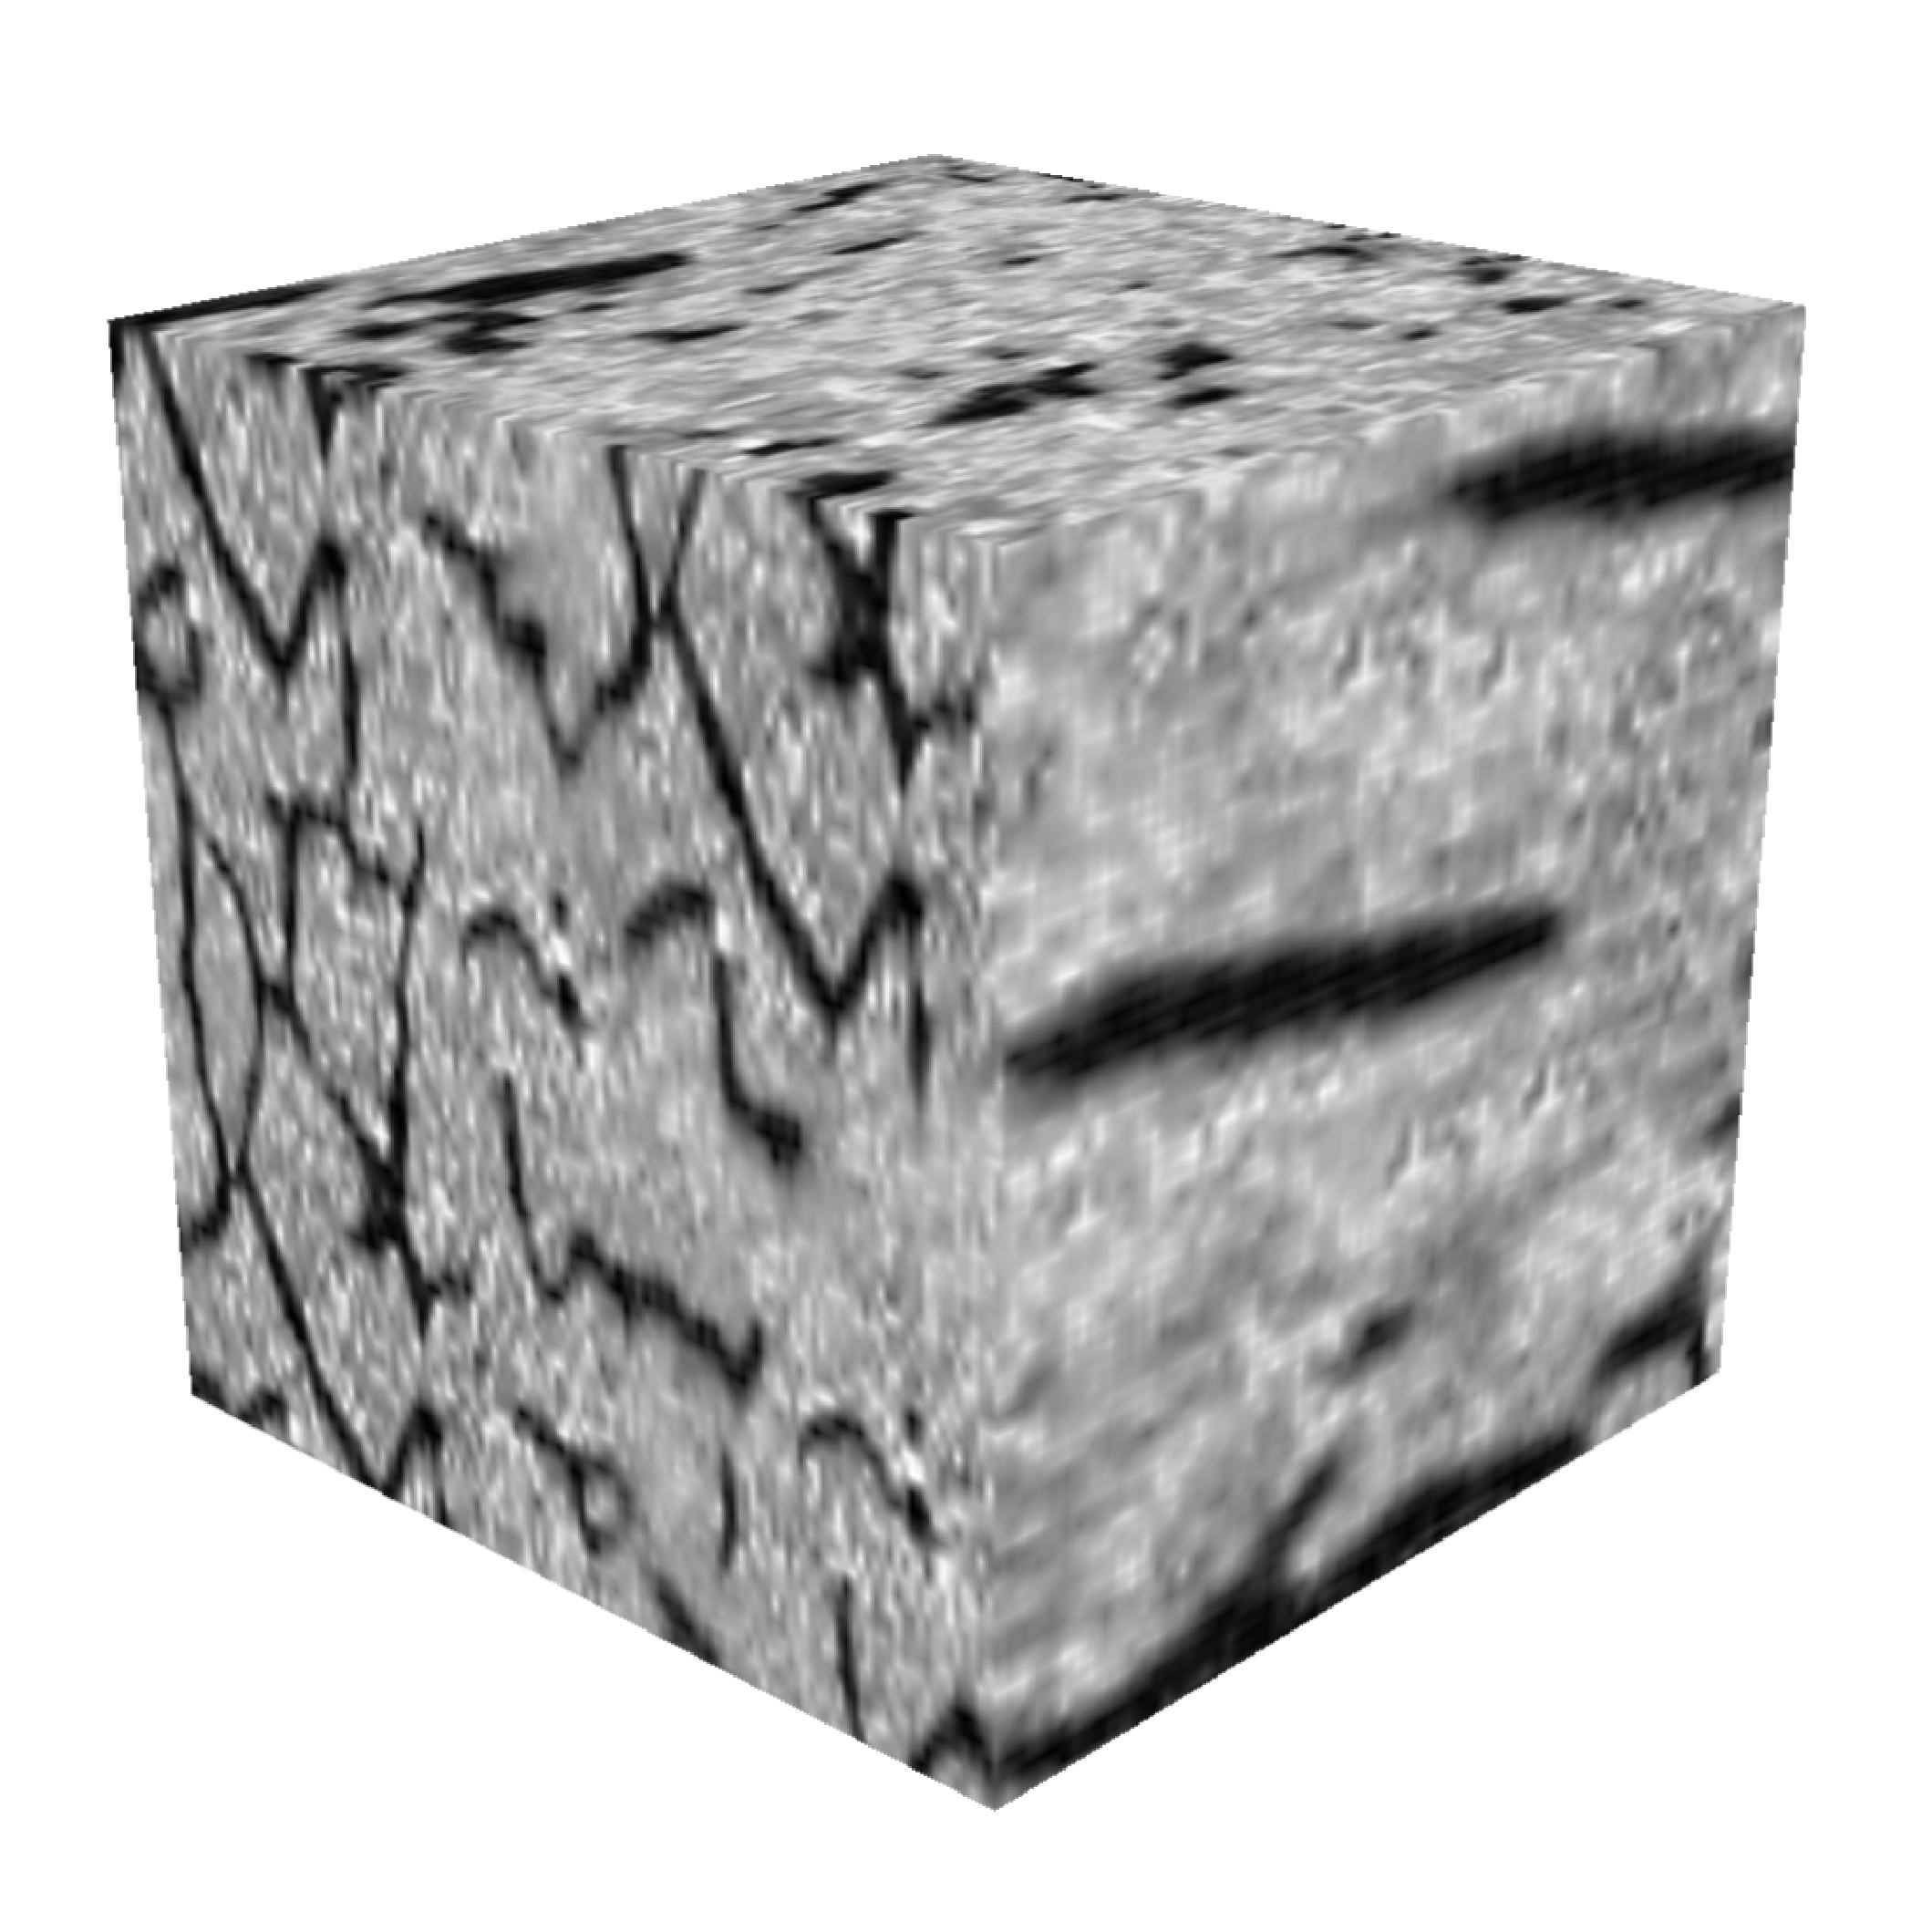
\epsfig{file = ModelIRM.eps, width = 3cm}
      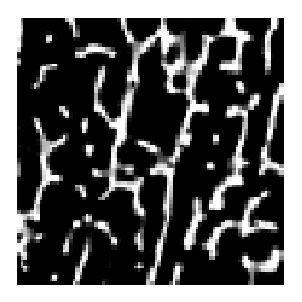
\epsfig{file = 42.irm_Y_015.eps, width = 2cm}
	    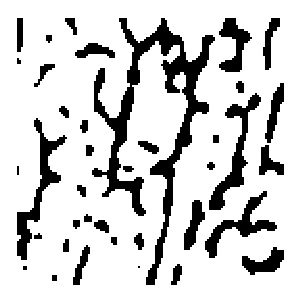
\epsfig{file = 42.irm_Y_015Mask.eps, width = 1cm}            
	    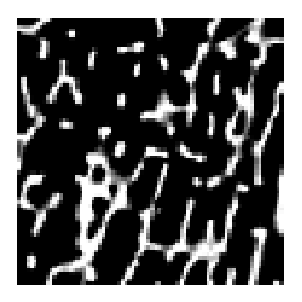
\epsfig{file = 42.irm_Y_047.eps, width = 2cm}
	    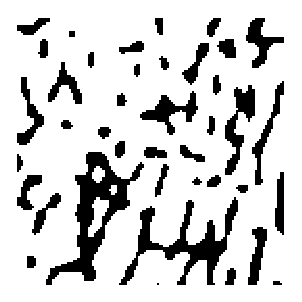
\epsfig{file = 42.irm_Y_047Mask.eps, width = 1cm}
	    \hspace{0.5cm}
	    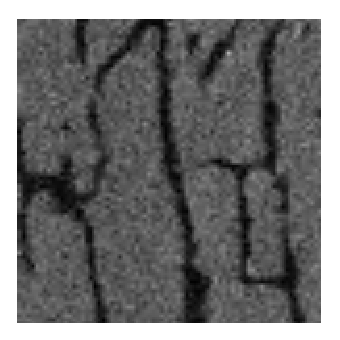
\epsfig{file = vol.73-93-94-sliceX.eps, width = 2cm}
	    
\epsfig{file = vol.73-93-94-sliceXMask.eps, width = 1cm}                        
	    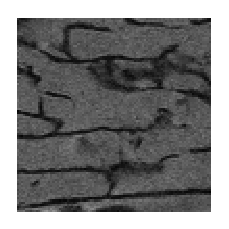
\epsfig{file = vol.73-93-94-sliceZ.eps, width = 2cm} 
	    
\epsfig{file = vol.73-93-94-sliceZMask.eps, width = 1cm}}\\
 \subfigure[3D virtual images.]{
 			\label{fig:ResultVolumes_textures}
 			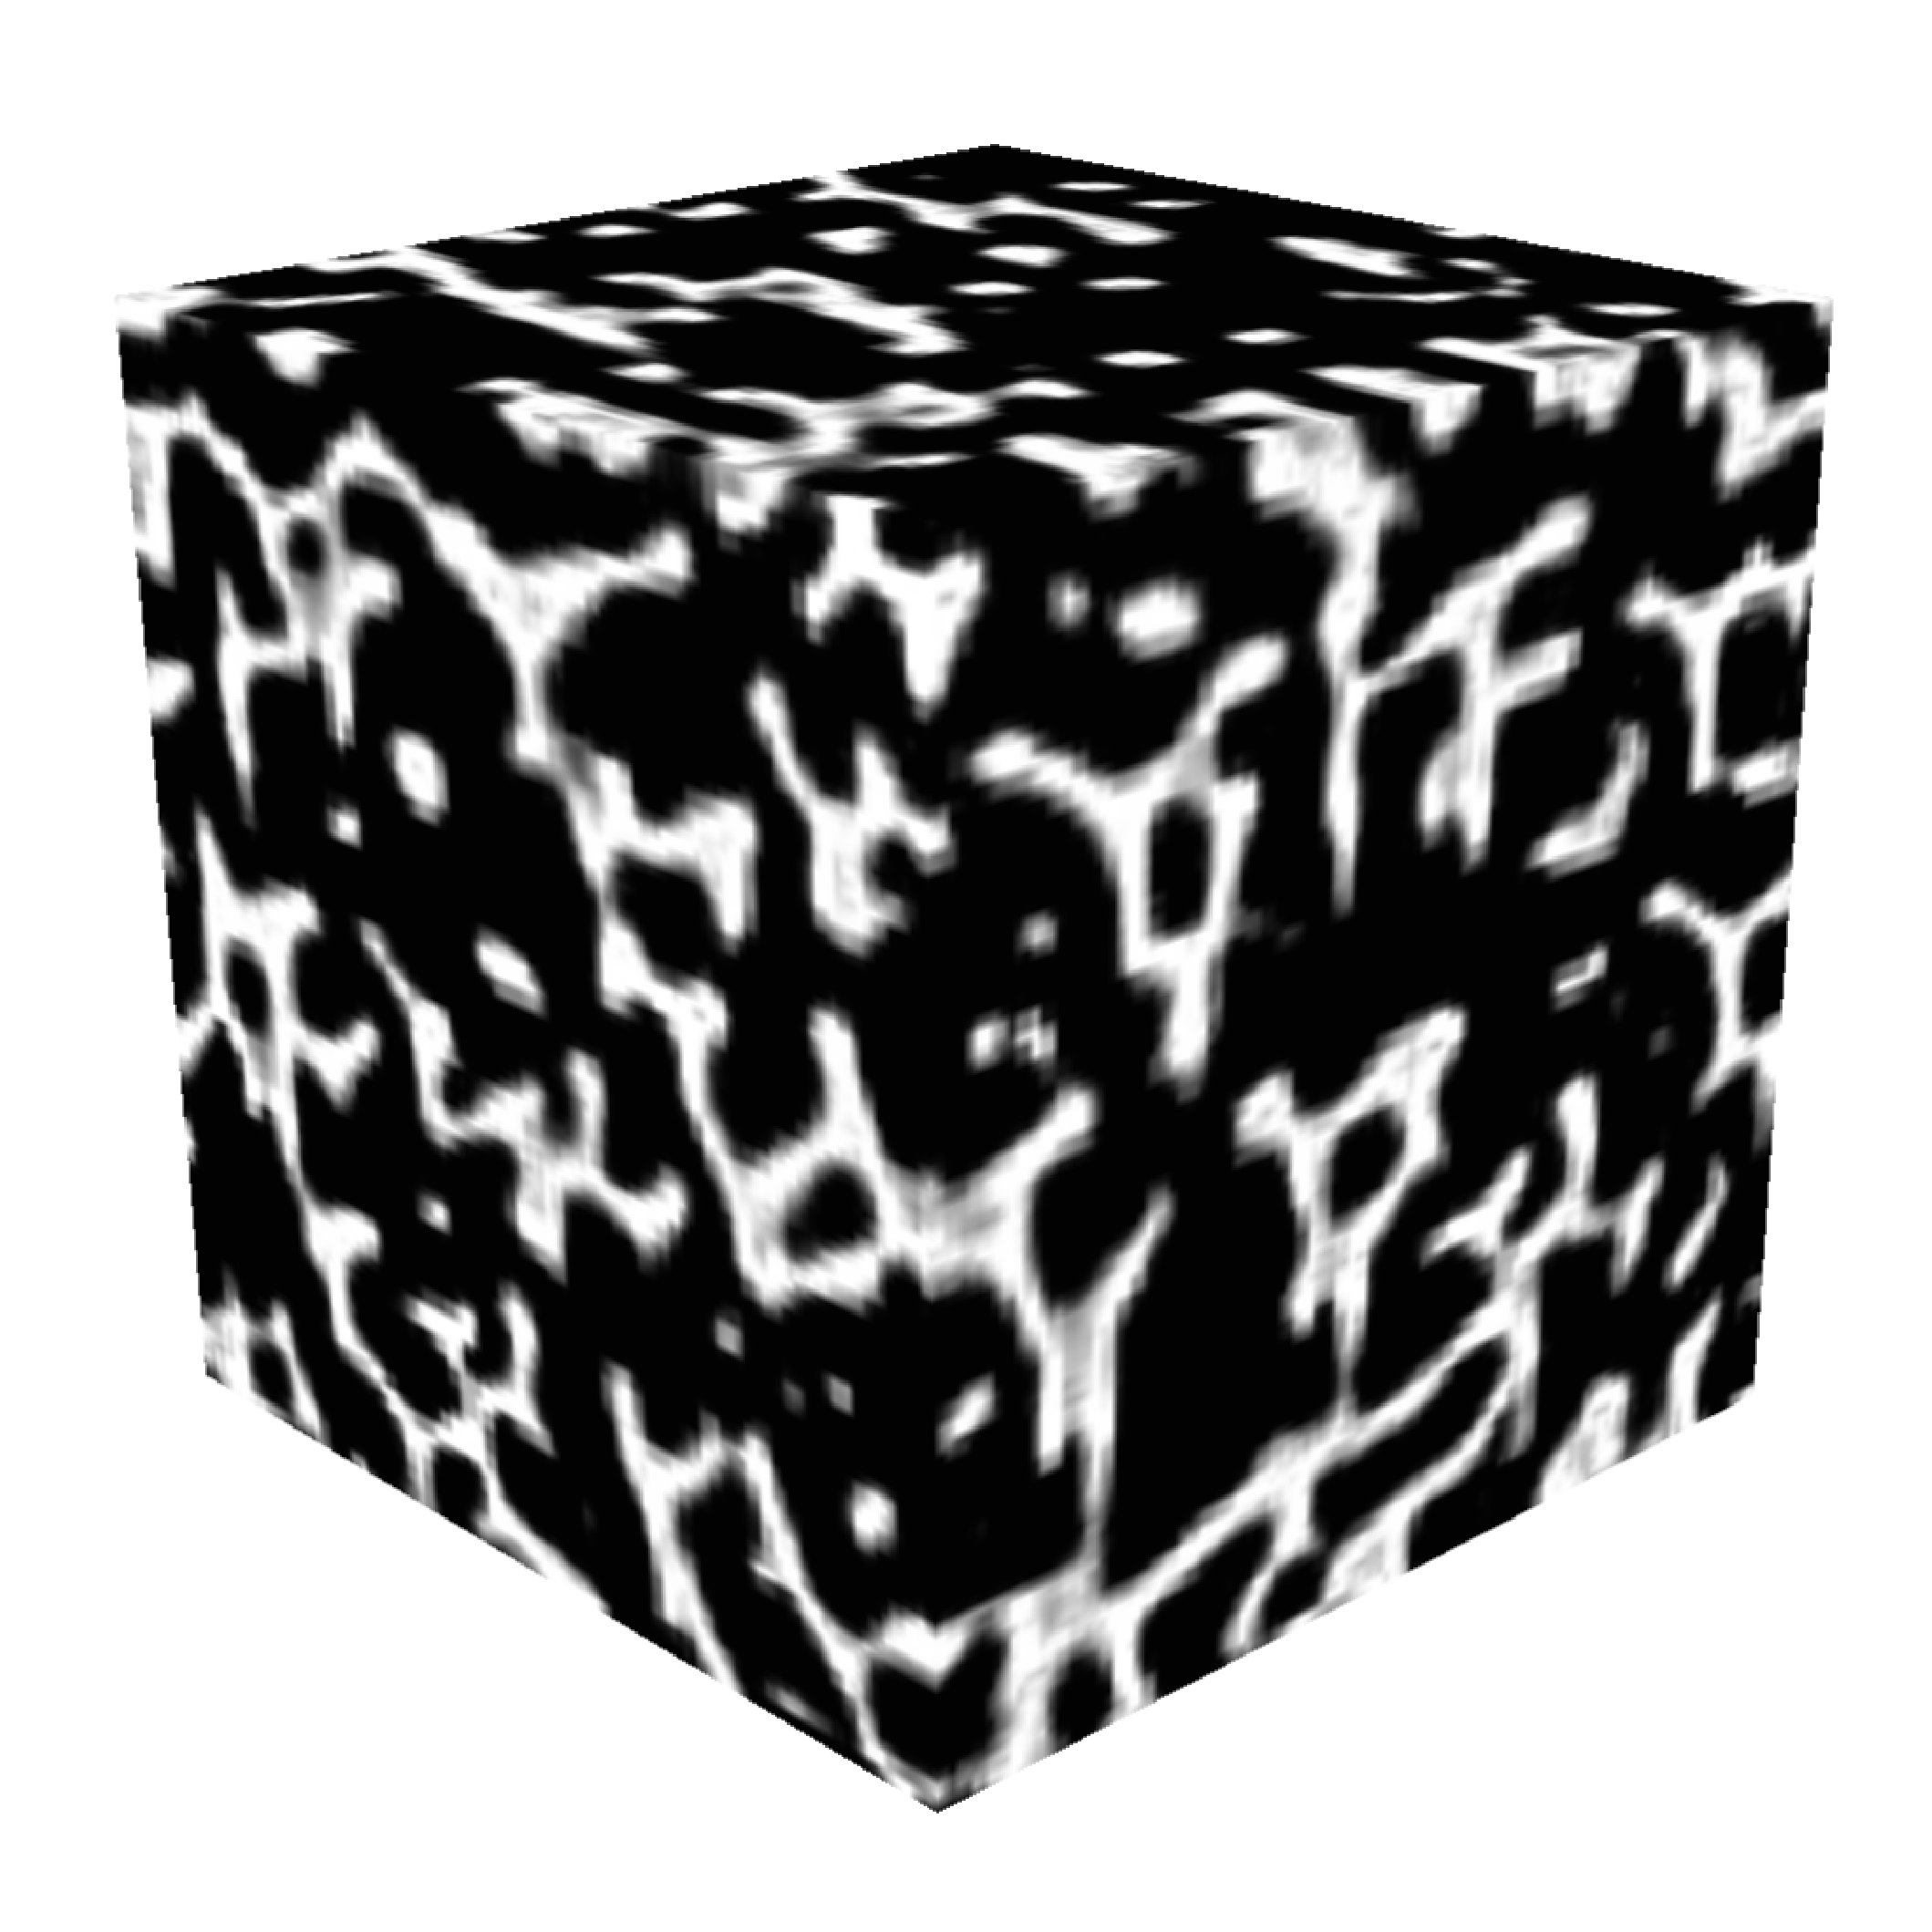
\epsfig{file = ModelESRF.eps, width = 7cm}
			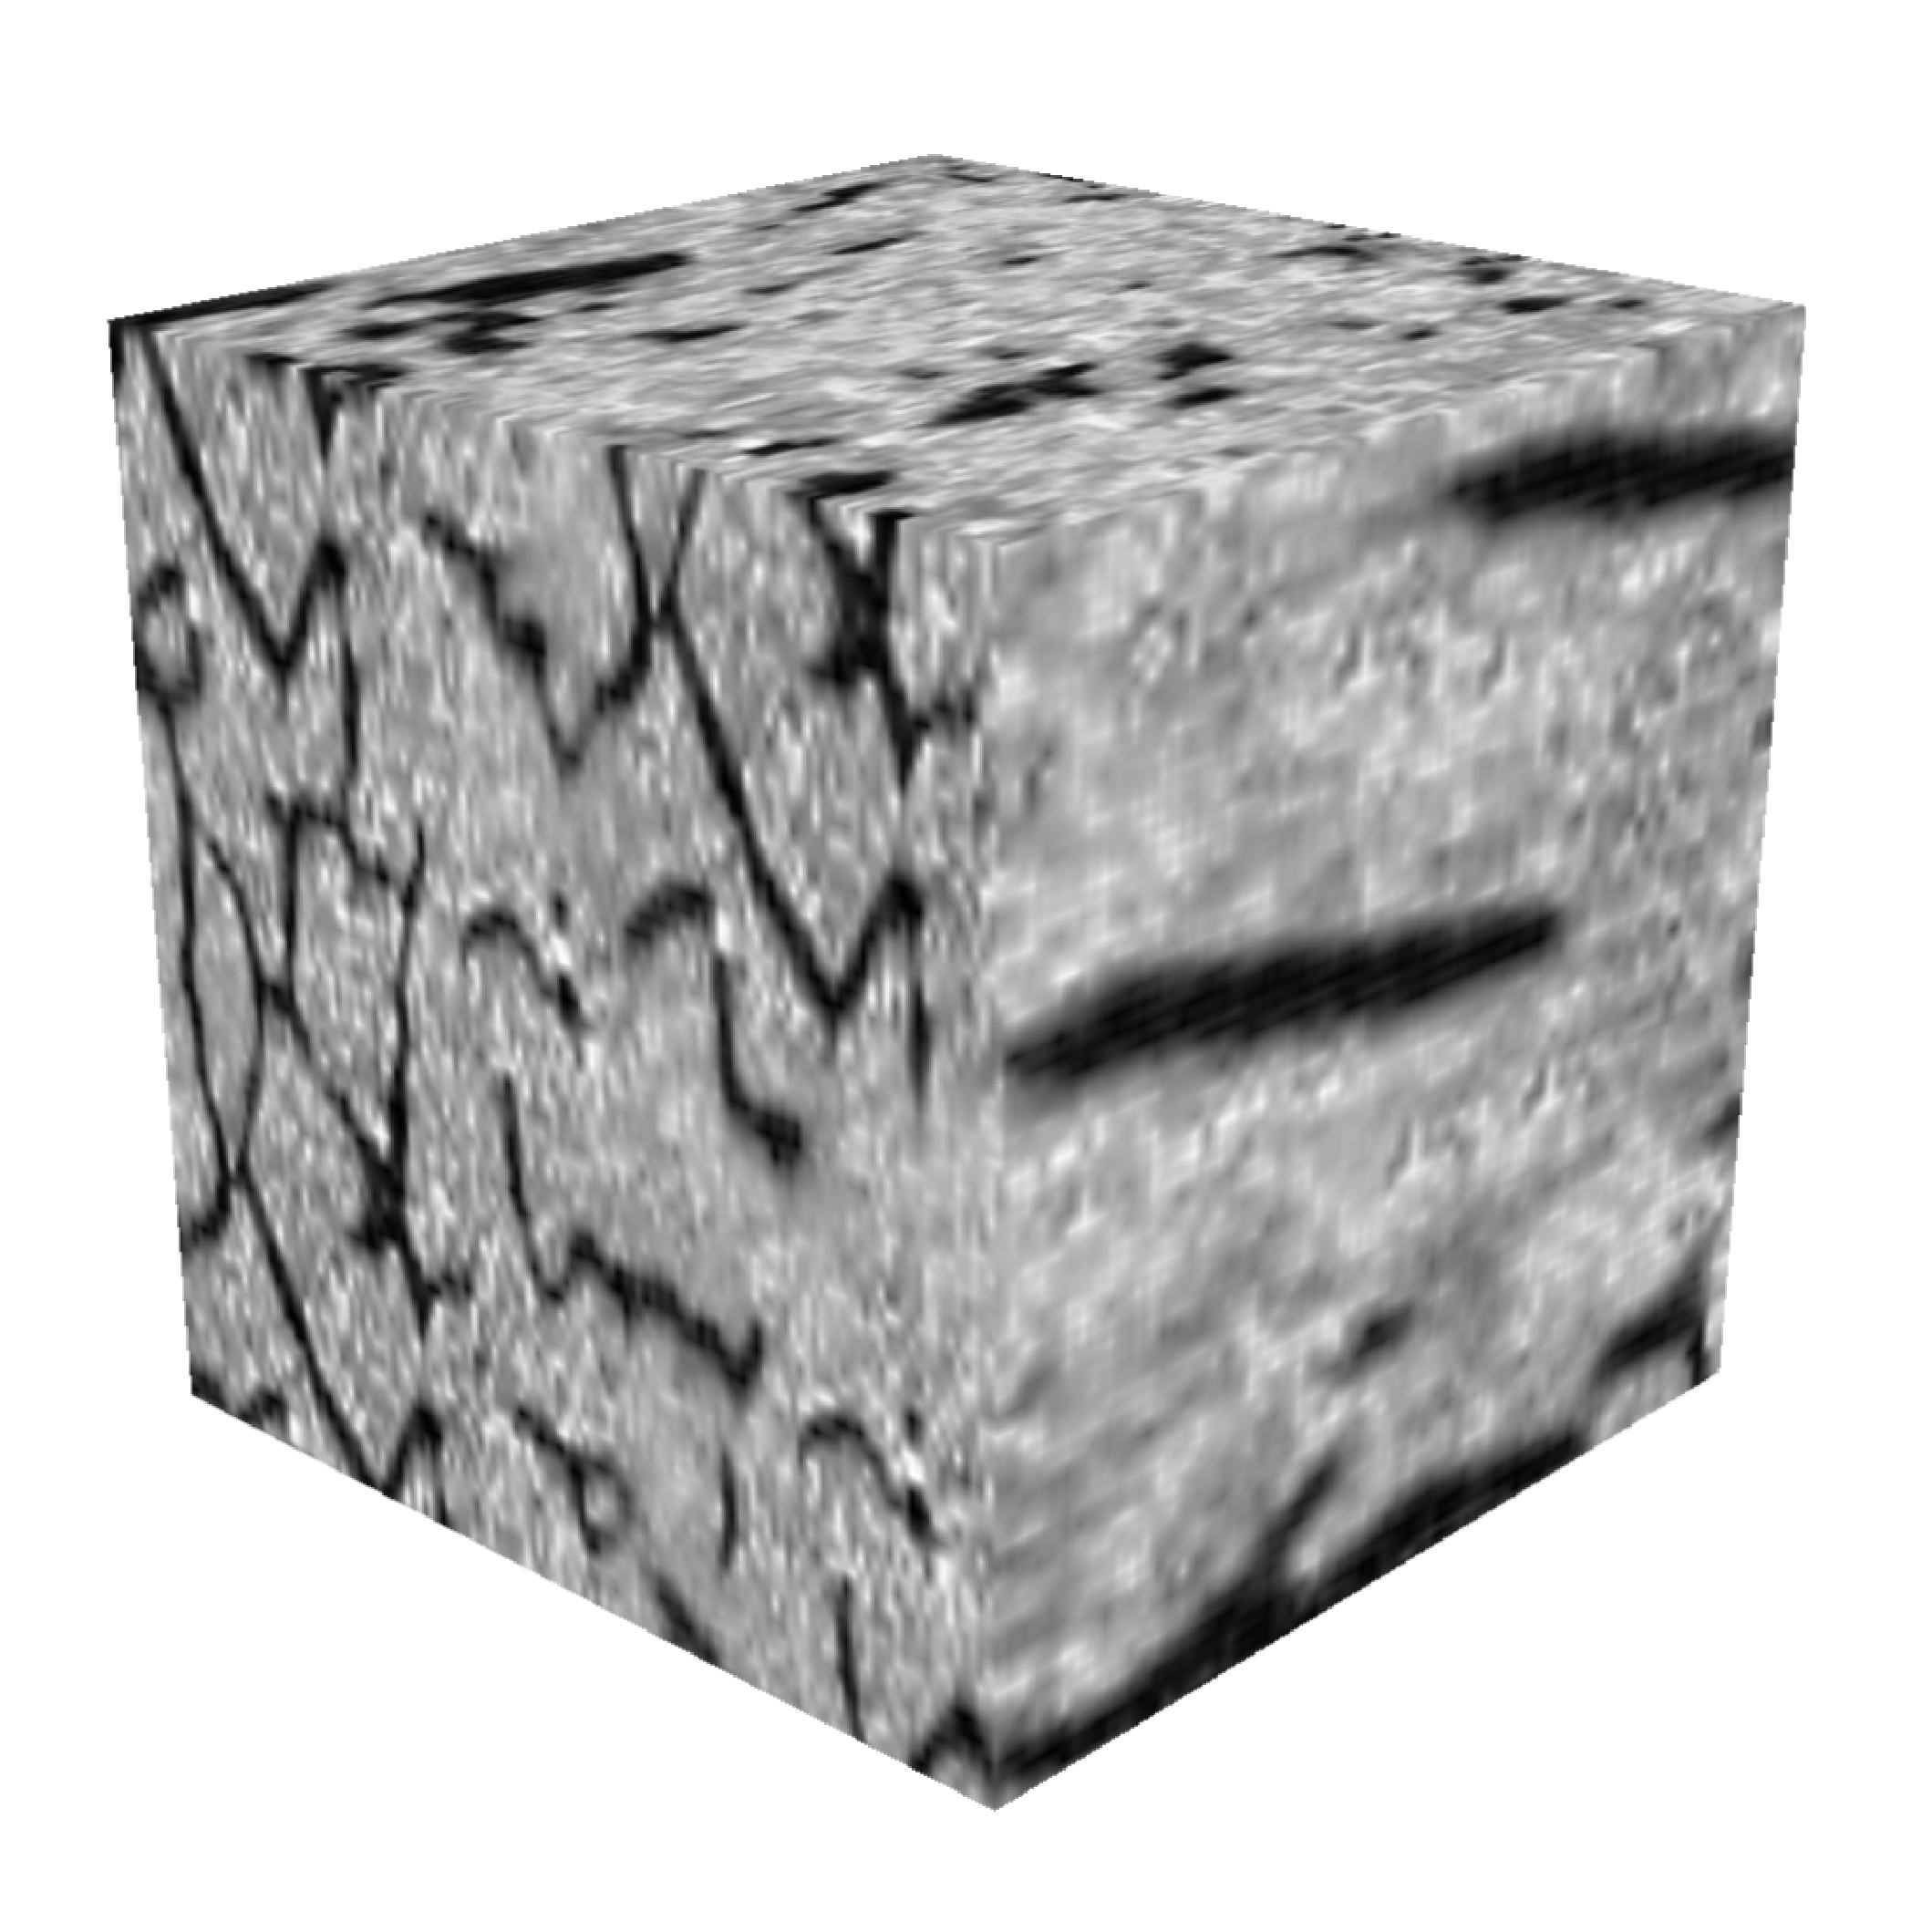
\epsfig{file = ModelIRM.eps, width = 7cm}
			      } 
 \caption[$SR \mu{CT}$ and $\mu{MRI}$ synthesis.]{Results of synthesis for $SR \mu{CT}$ (left) and $\mu{MRI}$ (right) using multiple textures to constrain plans perpendicular to axis-directions and binary masks to enhance the untextured areas.
         }
 \label{fig:ResultVolumesMRI_CT} 
\end{figure}

\begin{figure}[h!] 
 \centering
 %\subfigure[Exemplars + binary masks]{\epsfig{file = esrf.eps, width = 1cm}  
 %	    \epsfig{file = esrfMask.eps, width = 1cm} \hspace{1cm}
 %	    \epsfig{file = esrf1.eps, width = 1cm} 
 %	    \epsfig{file = esrf1Mask.eps, width = 1cm}
 %	   }
\subfigure[Synthetic volume.]{
			      \epsfig{file = texture3D-SRCTSynthetic.eps, width = 7cm}
			    }
\subfigure[Real volume.]{
			      \epsfig{file = texture3D-SRCT.eps, width = 7cm}
			     }
 \caption[Surface rendering of $SR \mu{CT}$ trabecular bone.]{Surface rendering of trabecular bone architecture obtained with the synthetic texture and the SR$\mu$CT image.}
 \label{fig:bone_surface_renderingMuCT} 
\end{figure}

\begin{figure}[h!] 
 \centering 
\subfigure[Synthetic volume.]{
			      \epsfig{file = IRM_synth_4_074.eps, width = 7cm}
			     }
\subfigure[Real volume.]{
			      \epsfig{file = IRM_Original_43.eps, width = 7cm}
			    }
 \caption[Surface rendering of $\mu$MR trabecular bone.]{Surface rendering of trabecular bone architecture obtained with: a) virtual $\mu$MR image, b) real $\mu$MR image.}
 \label{fig:bone_surface_renderingIRM} 
\end{figure}

\section{Evaluation of the synthesized textures}
\label{sec:EvaluationTexture}

To assess the quality of the synthetic 3D texture, 
statistical and morphological criteria are used.
As the ultimate goal is to produce a 3D texture as close as possible to the reference object, 
a comparison of statistical and morphological features between the reference and synthetic object 
is done.

\subsection{Statistical assessment}
\label{sec:StatisticsTexture}

\begin{table}[h]
\centering
\begin{tabular}{|c|c|c|c|c|c|c|}
  \hline
  & & Mean & St. Dev & Min & Max & Mode\\
  \hline
  \multirow{2}{*}{Red} & $e$ & 189.6  & 34.7  & 45 & 255 & 148 (253) \\
		       & $o$ & 188.7 & 34.0 & 48 & 255 & 146 (33562)\\
  \hline
  \multirow{2}{*}{Green} & $e$ & 142.4 & 70.2 & 21 & 255 & 255 (189)\\
		         & $o$ & 141.4 & 69.3 & 21 & 253 & 253 (27571)\\
  \hline
  \multirow{2}{*}{Blue} & $e$ & 168.8  & 48.7 & 51 & 254 & 108 (207)\\
		        & $o$ & 168.0  & 48.1 & 51 & 252 & 102 (26765) \\
  \hline
\end{tabular}
\caption{Means and standard deviations for the RGB channels of the exemplar and the object}
\label{tab:statshisto} 
\end{table}

Figure \ref{fig:histogramsHisto} shows the histograms from the muscle exemplar texture and the synthesized object shown 
in Figure \ref{fig:isotropicsynthesis}. The total number of pixels in the texture are $128^2 = 16384$ and
$128^3 = 2097152$ for the volume. When a randomly chosen slice is taken from the volume, the global statistics are still preserved
except from sampling errors.
Table \ref{tab:statshisto} contains the means and the standard deviations calculated from the histograms, the values
from the object are similar to those of the exemplar with a variation lower than 1$\%$ for the means and lower than 2$\%$ for the standard deviations. 

\begin{figure}[h!]
 \centering  
 \subfigure[Exemplar]{\epsfig{file = redHistoSample.eps, width = 5cm} 
	    \epsfig{file = greenHistoSample.eps, width = 5cm}
	    \epsfig{file = blueHistoSample.eps, width = 5cm}
           }\\
 \subfigure[Object]{\epsfig{file = redHistoObject.eps, width = 5cm}
	    \epsfig{file = greenHistoObject.eps, width = 5cm}
	    \epsfig{file = blueHistoObject.eps, width = 5cm}
           }
 \caption[RGB histograms of exemplar and synthesized solid.]{RGB histograms of the exemplar and the object for the striated
          cardiac muscle shown in figure \ref{fig:isotropicsynthesis}.}
 \label{fig:histogramsHisto} 
\end{figure}


Figure \ref{fig:histogramsMuMR} shows the histograms of the exemplar texture and the synthetic 3D $\mu{MR}$ 
image shown in Figure \ref{fig:ResultVolumesMRI_CT}. 

Thanks to the histogram matching, 
the grey levels distribution of the marrow and the bone are quite similar in the virtual image and the reference image. 
The statistics displayed near each histogram (mean, standard deviation, mode) are also very close.

\begin{figure}[h!]
 \centering 
 \subfigure[2D sample]{\epsfig{file = HistoSampleIRM.eps, width = 7cm}}
 \subfigure[3D synthetic image]{\epsfig{file = HistoModelIRM.eps, width = 7cm}}
\caption[Histogram comparison: $\mu{MR}$]{Comparison of the histograms obtained from the reference 2D and the 3D synthetic $\mu{MR}$ image.}
 \label{fig:histogramsMuMR}
\end{figure}


The histograms of the exemplars and solids for the physical parameters are created 
using 256 bins. Figure \ref{fig:histogramsPhysical} shows the histograms for the 
exemplars and synthesized volumes of physical parameters of the hippocampus. 
Global statistics are similar to the exemplar and shows the flexibility of the method
to work with images having multiple components. 

\begin{figure}[h!]
 \centering 
 \subfigure[$T_1$ 2D sample.]{\epsfig{file = histogramT1Exemplar.eps, width = 7cm}}
 \subfigure[$T_1$ 3D volume.]{\epsfig{file = histogramT1Volume.eps, width = 7cm}}
 \subfigure[$T_2$ 2D sample.]{\epsfig{file = histogramT2Exemplar.eps, width = 7cm}}
 \subfigure[$T_2$ 3D volume.]{\epsfig{file = histogramT2Volume.eps, width = 7cm}}
 \subfigure[$T_2^*$ 2D sample.]{\epsfig{file = histogramT2StarExemplar.eps, width = 7cm}}
 \subfigure[$T_2^*$ 3D volume.]{\epsfig{file = histogramT2StarVolume.eps, width = 7cm}}
 \subfigure[$M0$ 2D sample.]{\epsfig{file = histogramRhoExemplar.eps, width = 7cm}}
 \subfigure[$M0$ 3D volume.]{\epsfig{file = histogramRhoVolume.eps, width = 7cm}} 
\caption[Histogram comparison: physical parameters.]{Comparison of the histograms obtained from the 2D exemplar (left)
                                                     and the 3D volume (right) of physical parameters for the hippocampus
                                                    shown in Figure \ref{fig:isotropicsynthesisPhysical}.}
 \label{fig:histogramsPhysical}
\end{figure}



\subsection{Morphological assessment}
\label{sec:Morphology}

We propose to quantitatively assess the accuracy of the morphological structure given by the 
synthetic 3D texture. 
The method, software and original data sets used in this section were created by \cite{revol2002}.
For this study, %we\footnote{Chantal Muller and Juan Carlos Prieto} use 
3D textured images provided by Synchrotron Radiation Computed Micro-Tomography (SR$\mu$CT) were used.
These images were acquired some years ago on beam-line ID19 at the European Synchrotron Radiation Facility 
(ESRF) in Grenoble for the needs of a study focused on osteoporosis. 
Osteoporosis is a bone fragility disease leading to spontaneous bone fractures and 
characterized by a bone mass reduction and a bone structure deterioration. 
3D Synchrotron Radiation Computed Micro-Tomography (SR$\mu$CT) provided 3D high resolution 
images with an isotropic voxel of 10 $\mu$m width and a volume size of 
$330 \times 330 \times 330$ pixels can be used to assess trabecular bone architecture \cite{revol2002}. 
We have at our disposal a set of twelve 3D SR$\mu$CT images obtained from 
twelve calcaneus bone samples excavated from deceased human. 
For the test of my method, we worked on decimated SR$\mu$CT images with a resolution of 
80$\mu$m and a size of $83 \times 83 \times 83$ voxels. 
At this resolution, the signal to noise ratio is still high enough to extract trabecular 
bone from the background by simple automated thresholding. 
This binarizing step is needed for the computation of the bone parameters.

\begin{figure}[h!]
 \centering  
 \subfigure{\epsfig{file = esrfEvaluation.eps, width = 10cm}}
 \caption[Morphological evaluation of SR$\mu$CT texture.]{Box plots for morphologic and topological architecture of bone samples in SR$\mu$CT images. The syntetic 
          texture is displayed on the scale line under each box plot by a long red line.}
 \label{fig:bone_parametresMuCT} 
\end{figure}

We computed morphologic and topological architecture parameters similar to those used in histomorphometry 
but computed on three-dimensional images from the set of the twelve volumes. 
A 3D MIL (Mean Intercept Length) method based on a three-dimensional version of the directed 
secant algorithm was chosen to produce many parameters related to the trabecular 
bone morphology \cite{Hipp97} and the Euler number was computed to estimate the bone topology. 
We considered the seven following parameters: Partial Bone Volume (BV/TV), Bone Surface to 
Bone Volume ratio (BS/BV), Trabecular Thickness (Tb. Th), Trabecular Number (Tb. N), 
Trabecular Separation (Tb. Sp) and Mean Intercept Length (MIL1). The connectivity was estimated by the Euler number 
(Euler/mm3) implemented following the method described in 
\cite{Odgaard93} and normalized by the total volume. 
The higher the Euler number's value, the less connected the bone structure is.

3D SR$\mu$CT-like texture ($128 \times 128 \times 128$ voxels) was generated from two random 
reference slices ($83 \times 83$ pixels) taken from one of the twelve SR$\mu$CT volumes.  
We binarized the texture in order to extract the virtual bone architecture by the same automated 
thresholding that was used for the set of SR$\mu$CT volumes. 
We assess the accuracy of the virtual bone structure by comparing the bone parameters computed 
from the set of SR$\mu$CT images with those computed from the synthetic 3D volume.

Figure \ref{fig:bone_parametresMuCT} displays the box plots associated to each bone parameter obtained 
from the set of SR$\mu$CT images. As our aim is not focused on the analysis or 
the interpretation of these parameters but only on the comparison of them, 
we normalized each parameter by the range between their maximum and minimum values. 
The score of the synthetic texture is displayed on the scale line under each box plot by a 
long red line. All the morphological parameters of the
virtual bone spread in a range lower than +/- one standard deviation from the mean 
value obtained from the SR$\mu$CT. 
For the topology parameter (Euler/mm3), the score is higher than the maximum value 
obtained with the SR$\mu$CT set. It means that the synthetic bone 
structure has a lower connectivity than the reference set and could represent a high degree of osteoporosis.  

Figure \ref{fig:bone_surface_renderingMuCT} shows a comparison of the surface of the virtual bone and 
the 3D SR$\mu$CT image.
The surface of the syntetic bone is smoother that the real one.

A similar evaluation of the texture is done using $\mu$MR images.

\begin{figure}[h!]
 \centering 
 \subfigure{\epsfig{file = eval_morphologique_IRM_2.eps, width = 10cm}} 
\caption[Morphological evaluation of $\mu$MR texture.]{Boxplots of morphological and topological bone parameters computed from real and synthetic $\mu$MR images.}
 \label{fig:bone_parametresMuMR}
\end{figure}

The accuracy of the virtual images is assessed by comparing the bone parameters computed from the set of 
$\mu$MR images with those computed from synthetic ones.
Figure \ref{fig:bone_parametresMuMR} displays the boxplots associated to each bone parameter obtained from the sets of real 
and virtual $\mu$MR images. 

Figure \ref{fig:bone_surface_renderingIRM} shows the segmented trabecular bones from the 3D virtual $\mu$MR images and those obtained from the 3D $\mu$MR image 
from which were taken the reference slices for the texture synthesis. 
Once again the syntetic structure is smoother than the original sample image.


\section{Conclusion}
\label{sec:Conclusions}

The method allows one to create organic tissue from small samples acquired by a digital microscope or
other image acquisition devices such as SR$\mu$CT, $\mu$MR. %or relaxometry techniques.
The quality of the textures was demonstrated 
quantitatively from both statistical and morphological points of view.
The morphological analysis showed a lower quality of synthesized bone.

This texture synthesis approach is able to preserve the statistical information 
with accuracy and the morphology of the given sample in a lower degree.
Even though the computed morphological parameters were 
inside the range of plausible values, the quality of the bone is degraded.  
If the synthesized volumetric object must preserve structure, a procedural approach 
to synthesize texture might be a better option than the approaches using 2D samples of texture.
As mentioned in the introduction of this chapter, procedural approaches are difficult to parameterize. 

%Latter tests showed that the zebra-dot 3D texture can be useful for simulation especially in the framework of Brownian simulation.
The following chapter explains MRI simulation and
the procedure to acquire the textured samples 
for some brain structures. 
To produced simulated MRI, textured samples containing information of physical parameters are used.
These samples of physical parameters do not contain structural information, so 
the proposed approach can be used to produced volumes of physical parameters.

The solid textures are combined 
with s-reps (see Section \ref{sec:solidRep}) to enhance their properties 
and enable MRI simulation.


\newpage

